\chapter{Алгоритм численного исследования упрощённой модели}  \label{Numer}
К сожалению, авторами не придумано аналитического способа решения поставленной задачи в терминах операторов \eqref{eq:Investigated_linear_operator} или даже \eqref{eq:Local_operator_definition}. Однако стремление исследовать локальную задачу для функции Грина \eqref{eq:Local_operator_Green_function_definition} основано на том, что для неё существует мощный метод численного исследований вопроса, который мы далее опишем. Также этот метод позволяет исследовать статистику решения уравнения самосогласования, что нами также будет проделано.



\section{Теория алгоритма популяционной динамики}
В данной секции будет дано краткое теоретическое обоснование и формулировка численного алгоритма для исследования локальных задач на регулярных графах.


\subsection{Связь свойств большого $K$-регулярного со свойствами деревьев с постоянными числом ветвления}
Большие $K$-регулярные графы обладают следующим набором полезных свойств, которые позволяют их на физическом уровне строгости считать не содержащими циклов. Более детально, рассуждение выглядит следующим образом:
\begin{itemize}
	\item Математически строгим фактом является следующее утверждение: среднее число циклов в большом регулярном графе является некоторой константой и не зависит от его размера в термодинамическом пределе $M \rightarrow \infty$. Формально, на уровне теоремы, это выглядит так: рассмотрим последовательность ансамблей $R(M)$ случайных графов размера $M$ с заданным числом ветвления $K$. Обозначим через $\left\langle \cdot \right\rangle_M$ среднее от некоторой величины по ансамблю $R(M)$, а через $c_k$ обозначим число циклов длины $k$ в заданном графе. Тогда
	\begin{equation}
		\label{eq:Theorem_average_number_of_cycles}
		\forall k > 0 \hookrightarrow \left\langle c_k \right\rangle_M = \frac{K^k}{2k} \left(1 + o(1) \right), M \rightarrow \infty 
	\end{equation}
	Доказательство этого утверждения можно восстановить по \cite{McKay_1981}. 
	
	\item Физическая интерпретация этой теоремы состоит в том, что вероятность у случайно выбранного узла принадлежать циклу заданной длины в термодинамическом пределе равна нулю: действительно, число узлов, лежащих в каком-нибудь цикле длины $k$ в термодинамическом пределе является постоянным числом $K^k / 2$, так что доля таких узлов во все системе исчезающе мала.
	
	\item Очевидным следствием будет следующее утверждение про некоторое подмножество узлов небольшого радиуса: вероятность того, что внутри этого подмножества содержится \textit{какой-либо цикл}, также равна нулю в термодинамическом пределе. Это свойство носит название \textit{локально древовидной структуры}.
	
	\item Важное физическое проявление указанного свойства состоит в том, что все физические величины, обладающие конечной характерной длиной, не будут различать достаточно большой $K$-регулярный граф и дерево с постоянным числом ветвления $K$. Такими величинами являются, например, свойства волновых функций в локализованной фазе, все характеристики конечных систем, а также все характеристики системы на конечной частоте \cite{Tikhonov_2016}.
\end{itemize}
Далее мы будем активно пользоваться этими рассуждениями, а именно, мы предположим, что в рассматриваемом нами графе нету циклов, т. е. он является деревом. Здесь необходимо сделать некоторые физические комментарии:
\begin{itemize}
	\item Разумеется, роль циклов в нелокальных свойствах весьма существенна. Например, исследование задач буквально на деревьях требует очень аккуратного обращения с граничными условиями, поскольку на дереве граница даёт доминирующий вклад в общий объём системы, в то время как на больших регулярных графах выполнение правильных граничных условий самосогласованно обеспечивается именно циклами размерами порядка диаметра системы. В частности, известно \cite{Tikhonov_2016}, что у статистики свойств состояний и уровней энергии в делокализованной фазе наблюдаются существенные качественные различие в случае дерева и регулярного графа. Поэтому в исследуемых нами системах необходимо озаботиться механизмами, гарантирующих правильное поведение подобных величин.
	
	\item Также заметим, что замена случайного регулярного графа на дерево по сути является способом избавиться от беспорядка, вносимого распределением ансамбля $K$-регулярных графов.
	
	\item Замена большого регулярного графа на дерево с постоянным числом ветвления с дополнительными условиями самосогласования также может быть рассмотрена в терминах реплично-симметричного приближения и соответствующей седловой точки некоторого функциональньного интеграла, что проделано в работе \cite{Metz_Castillo_2017}.
\end{itemize}


\subsection{Вывод уравнений популяционной динамики}
Итак, перед нами стоит задача вычисления статистики диагональных элементов функции Грина \eqref{eq:Local_operator_Green_function_definition} для оператора $C$, живущего теперь уже на дереве. Для \textit{статистики} буквально в этой задаче существует мощная численная процедура, называемая \textit{методом популяционной динамики}. Она уже неоднократно использовалась для изучения задач одночастичной Андерсоновской локализации \cite{Biroli_2010} и показала себя крайне эффективно. Далее мы продемонстрируем обоснование и некоторые полезные свойства этого метода на основании работы \cite{Rogers_2008}.

\subsubsection{Обозначения}
Примем ряд обозначений для дальнейшего изложения (большинство из них нужны лишь для записи вывода основных результатов и не потребуются для использования и обсуждения этих результатов):
\begin{enumerate}
	\item Далее мы будем обозначать одинаково граф, множество его узлов, рёбер и прочие характеристики --- из контекста всегда будет понятно, о чем идёт речь. 
	
	\item Кроме самого графа $T$ исходной системы нам также понадобится граф $T[j]$, получаемы из исходного удалением вершины $j$ (и, соответственно, всех смежных ей рёбер).
	
	\item Для нас существенен следующий факт: если граф $T$ был деревом, то все графы $T[j]$ будут набором несвязанных деревьев, каждое из которых можно быть однозначно задано своим корнем $k \in \partial j$, являющимся одним из непосредственных удалённого узла $j$ в исходном дереве. Эти новые поддеревья мы обозначим как $T[j]\{k\}$
	
	\item Далее мы будем вычислять некоторые функции $f$ для заданного графа $T$. Если это делается для графов $T[j]$ или $T[j]\{k\}$, то мы будем такие характеристики обозначать, соответственно, как $f[j], f[j]\{k\}$.
	
	\item В частности, для некоторого узла $i \in T$ графа мы будем обозначать множество его соседей как
	$$
	\left\{ k : \langle ik \rangle \in T \right\} \equiv \partial i
	$$
	Если речь будет идти о графах $T[j],T[j]\{k\}$, то границу мы будем обозначать соответственно $\partial[j]i, \partial[j]\{k\}i$
		
\end{enumerate}

\subsubsection{Определение локальных полей}
Итак, пусть у нас имеется некоторое дерево или система деревьев $T$, и нас интересуют диагональные элементы функции Грина вида
$$
G(\mu = 1 + i0)_{ii} := \left( \mu - \hat{C} \right)^{-1}_{ii} 
$$
где матрица $\hat{C}$ выражается через матрицу смежности графа $T$ посредством определения \eqref{eq:Local_operator_definition}. Для нас существенно, что у матрицы $C$ множество индексов ненулевых элементов является подмножеством множества таких индексов для матрицы смежности графа $T$. Далее дадим следующи ряд определений:
\begin{itemize}
	\item Введём на каждом узле $i$ графа некоторое вещественное поле $\phi_i \in \mathbb{R}$ и рассмотрим ансамбль значений этих полей, задаваемых следующим весом:
	\begin{equation}
	\label{eq:Cavity_method_generating_function}
	P\{\phi\} := \exp\left\{ \frac{i}{2} \left(\mu\sum_{i \in T}\phi_i^{2} - \sum_{i,j \in T} \phi_i C_{ij} \phi_j \right)\right\} 
	\end{equation}
	
	\item Определим также стат. сумму этого распределения
	\begin{equation}
	\label{eq:Cavity_method_partition_function_definition}
	Z := \int \left( \prod_{k \in T} d\phi_k \right) P\{\phi\}
	\end{equation}
	
	\item Среднее от некоторой функции значения полей $f\left( \{\phi\} \right)$ определяется как
	\begin{equation}
	\label{eq:Cavity_method_average_definition}
	\left\langle f \right\rangle = \frac{1}{Z} \int \left( \prod_{k \in T} d\phi_k \right) f\left( \{\phi\} \right) P\{\phi\} 
	\end{equation}
	Поскольку у $\mu$ имеется положительная мнимая часть, то все интегралы являются сходящимися. 
	
	\item Элементы функции Грина $G$ могут быть выражены как
	\begin{equation}
	\label{eq:Cavity_method_Green_function_expression}
	G_{ij} = i \left\langle \phi_i \phi_j \right\rangle
	\end{equation}
	
	\item Также нам понадобятся функции одноузельных распределений введённых полей, определяемые как
	\begin{equation}
	\label{eq:Cavity_method_single_field_distribution_definition}
	p_i(x) := \left\langle \delta(\phi_i - x) \right\rangle
	\end{equation}
	
	\item Очевидным свойством является то, что одноузельные распределения содержат всю интересующую нас информацию о диагональных элементах функции Грина:
	\begin{equation}
	\label{eq:Cavity_method_GF_diagonal_elements_through_single_field_distrivution}
	G_{ii} = \int p_i(y) dy
	\end{equation}
	\item Как указано в начале, все эти определения и утверждения валидны также для $T[j], T[j]\{k\}$.
\end{itemize}
Отметим, что подход производящего функционала также может быть использован для аналитического исследования некоторого класса задача на графах методом реплик, что проделано, например, в \cite{Rodgers_Bray_1988}.

\subsubsection{Рекуррентные уравнения на одноузельные распределения}
Рассмотрим функции $p[j]_i(x)$ в системе с выкинутым узлом $j$. Прежде всего, заметим, что поскольку поддеревья $\left\{ T[j]\{i\}: i \in \partial j \right\}$ не связаны между собой рёбрами, то из определения $p$ тривиально следует равенство одноузельных распределений для узлов новых поддеревьев, если эти распределение вычислять во всей системе $T[j]$ и в отдельном поддереве $T[j]\{k\}$:
$$
i \in  T[j]\{k\} \Rightarrow p[j]_i(x) \equiv p[j]\{k\}_i(x)
$$
С другой стороны, определение $p[j]$ с помощью преобразований над весом усреднения \eqref{eq:Cavity_method_generating_function} позволяет показать следующее тожество для одноузельных распределений в корнях деревьев $T[j]\{k\}$:
\begin{equation}
	\label{eq:Single_field_cavity_distribution_recurrence_relation}
	p[j]\{k\}_k(x) = \frac{\exp\left\{ \frac{i}{2}\mu x^2\right\} }{Z[j]\{k\}} \prod\limits_{s \in \partial[j]k} \left[Z[k]\{s\} \int p[k]\{s\}_s(y) \exp\left\{ -i x y С_{sk} \right\} dy \right]
\end{equation}
Аналогичным образом можно установить связь между системой $T$ и $T[j]$
\begin{equation}
	\label{eq:Single_field_distribution_though_cavity_distributions}
	p_j(x) = \frac{\exp\left\{ \frac{i}{2}\mu x^2\right\} }{Z} \prod\limits_{k \in \partial j} \left[Z[k] \int p[j]_k(k) \exp\left\{ -i x y С_{jk} \right\} dy \right]
\end{equation}

\subsubsection{Рекуррентные уравнения на диагональные элементы функции Грина}
Следующим шагом будет заметить, что уравнения \eqref{eq:Single_field_cavity_distribution_recurrence_relation}-\eqref{eq:Single_field_distribution_though_cavity_distributions} допускают следующий анзатц:
\begin{equation}
	\label{eq:Single_site_distribution_gaussian_ansatz}
	p...(x) = A... \exp\left\{- \frac{x^2}{2 v...} \right\}, v... \in \mathbb{C}
\end{equation}
где $...$ - индексы, задающие граф и узел. Данный анзатц приводит к следующим уравнениям на величины $v$:
\begin{equation}
	\label{eq:Cavity_amplitude_recurrence_relation}
	v[j]_k = \left[ \sum_{s \in \partial[j]k} C_{ks}^{2} v[k]_s - i\mu \right]^{-1}
\end{equation}
\begin{equation}
	\label{eq:Dispersion_though_cavity_amplitudes}
	v_j = \left[ \sum_{k \in \partial j} C_{jk}^{2} v[j]_k - i\mu \right]^{-1}
\end{equation}
Заметим, что поскольку $\Im \mu > 0$, то можно показать, что данные рекуррентные уравнения сохраняют свойство $\Re v > 0$, так что все рассматриваемые интегралы являются Гауссовым образом сходящимися.

Наконец, важным наблюдением будет то, что гауссов анзатц \eqref{eq:Single_site_distribution_gaussian_ansatz} напрямую связан с желаемыми диагональными элементами функции Грина посредством уравнения \eqref{eq:Cavity_method_GF_diagonal_elements_through_single_field_distrivution}:
$$
G_{jj} \equiv i v_j
$$

Введём общепринятые для полученного метода обозначения:
$$
v[j]_k =: G_{j \rightarrow k}
$$
$$
i v_j =: G_j \equiv G_{jj}
$$
Тогда метод популяционной динамики формулируется как следующий набор рекуррентных уравнений:
\begin{equation}
	\label{eq:Population_dynamics_equations}
	\begin{split}
		G_{j \rightarrow k} & = \left[ \sum_{s \in \partial[j]k} C_{ks}^{2} G_{k \rightarrow s} - i\mu \right]^{-1} \\
		G_j & = i \left[ \sum_{k \in \partial j} C_{jk}^{2} G_{j \rightarrow k} - i\mu \right]^{-1}
	\end{split}
\end{equation}
Таким образом, система уравнений \eqref{eq:Population_dynamics_equations} является замкнутым способом определить значение диагональных элементов функции Грина \eqref{eq:Local_operator_Green_function_definition} на заданном древесном графе.

\subsubsection{Комментарии по использованию полученных уравнений}
На полученные рекуррентные уравнения может смотреть двумя способами:
\begin{itemize}
	\item во-первых, как на способ найти диагональную функцию Грина на любом узле графа \textit{в заданной реализации беспорядка} и \textit{без явной диагонализации соответствующей матрицы}. Здесь важно два аспекта:
	\begin{itemize}
		\item Во-первых, такая интерпретация явным образом указывает на разницу между деревом и регулярным графом: в первом случае указанные уравнения сопровождаются указанием граничных условия, в то время как во втором требуется условие согласования на всех циклах системы.
		\item Полученная система уравнений требует двух процедур рекурсии от краёв дерева к центру и обратно, причём можно показать, что алгоритм имеет сложность и затраты памяти $O(M)$, где $M$ --- число узлов. Это даёт огромный выигрыш по сравнению с методами диагонализации разреженных матриц, которые в лучшем случае требуют $O(M^2)$ времени и памяти. 
	\end{itemize}
	\item Во-вторых, можно интерпретировать эти рекуррентные соотношения как \textit{уравнения на распределения по ансамблю беспорядка}. Более конкретно, система \eqref{eq:Population_dynamics_equations} может быть переписана в замкнутое интегральное уравнение на распределение величин $P(G_{j \rightarrow k}), P(G_i)$ при известном распределении величин $\xi_i$, организующим в системе беспорядок. Здесь тоже сделаем два важных физических замечания
	\begin{itemize}
		\item Полученные численные уравнения в таком случае являются ничем иным, как способом итеративного численного решения указанного интегрального уравнения. В связи с этим заметим также, что возникающее таким образом уравнение на стационарную точку рекурсии в реальной системе на графе является следствием упомянутых уравнения самосогласования, возникающих в результате присутствия в системе циклов размером порядка диаметра графа. 
		\item Такой подход к этим уравнениями приводит к известным результатам по описанию локализации Андерсона \cite{AAT}. Обратим внимание, что это возможно только благодаря локально древовидной структуре графа. 
	\end{itemize}
\end{itemize}

Наконец, как уже отмечено в начале этой главы, нам нужно гарантировать, что получаемые нами, вообще говоря, нелокальные свойства, вроде плотности состояний на узле и IPR будут относиться именно к $K$-регулярному графу. В общем случае (т. е. если априори неизвестно, является ли фаза локализованной) это достигается правильным порядком предельного перехода по имеющимся параметрам: числу итераций рекурсии $N$, размеру системы $M$ и уширению уровней $\gamma$. Правильный порядок предельного перехода получается, если вспомнить, что ответы для деревьев и графов не отличаются для величин с некоторым конечным масштабом длины. При конечном значении регуляризации $\gamma$ такой характерной величиной будет длина $L_{char} \propto \ln \gamma^{-1}$, которую способна пролететь частица без диссипации \cite{Tikhonov_2016}. А значит, правильный порядок таков:
\begin{itemize}
	\item сначала необходимо найти стационарную точку уравнений рекурсий, обеспечив тем самым выполнение самосогласования за счёт больших циклов,
	\item затем требуется перейти к термодинамическому пределу бесконечной системы $M \rightarrow \infty$,
	\item и, наконец, взять предел $\gamma \rightarrow 0$.
\end{itemize}
Физически взятие этих пределов соответствует тому, что:
\begin{itemize}
	\item Число итераций метода должно быть много больше диаметра системы, чтобы гарантировано обойти все циклы: 
	$$N \gg d \sim \frac{ \ln M}{\ln K} $$
	\item размер системы $M$ должен много превышать объём, содержащий указанную характерную длину:
	$$
	M \gg K^{L_{char}} \sim \exp \left\{ \sharp \ln K \ln \frac{1}{\gamma} \right\}
	$$
	\item Оценку для характерного масштаба $\gamma$ провести из таких качественных рассуждений нельзя, однако существование данного предела определяется внутренними масштабами уравнений самосогласования, возникающих на циклах. 
\end{itemize}

\subsubsection{Эквивалентность задаче локализации Андерсона с диагональным беспорядком на дереве}
При конкретном виде \eqref{eq:Local_operator_definition} матрицы $C$ в уравнениях популяционной динамики \eqref{eq:Population_dynamics_equations} можно провести следующую замену:
\begin{equation}
\label{eq:Population_dynamics_change_of_variables}
G_{j \rightarrow k} \longmapsto \frac{ G_{j \rightarrow k} }{ \frac{g}{K} \eta_k}
\end{equation}
после которой уравнения приобретут вид
\begin{equation}
\label{eq:Population_dynamics_final_equations}
\begin{split}
\begin{split}
G_{j \rightarrow k} & = \left[ \frac{g}{K} \sum_{s \in \partial[j]k} G_{k \rightarrow s} - \frac{  i \mu}{\eta} \frac{K}{g} \right]^{-1} \\
G_j & = i \left[ \frac{g}{K} \eta \sum_{k \in \partial j} G_{j \rightarrow k} - i\mu \right]^{-1}
\end{split}
\end{split}
\end{equation}
Эта замена имеет очень большое значение, поскольку теперь первое уравнение \textit{идентично} тому, что возникает при изучении стандартной задачи локализации Андерсона с диагональным беспорядком в центре зоны \cite{Biroli_2010}. Это позволяет в дальнейшем применять к нашей модели многочисленные результаты теоретического исследования задачи Андерсона, полученные, например, в \cite{AAT}.


\subsection{Формулировка итоговой численной процедуры}
Приведём подробную формулировку численной процедуры метода популяционной динамики применительно к нашей задаче.

\subsubsection{Алгоритм популяционной динамики}
Сформулируем конкретную процедуру, которая далее авторами данной работы реализована на \textit{С++} и \textit{Wolfram Mathematica}. 
\begin{enumerate}
	\item \textit{Инициализация}: заводится два одинаково больших (размером $M \sim 10^{7} \div 10^{9}$) массива комплексных чисел $G_{i \rightarrow j}$, первый из них инициализируется случайными комплексными числами с $\Re G_{i \rightarrow j} > 0$. Первый массив помечается меткой текущего $cur$ а второй --- меткой обновляемого $upd$.
	
	\item \textit{Один шаг} метода состоит в следующем:
		\begin{itemize}
			\item в массиве $upd$ зафиксировать один элемент (его индекс)
			\item Выбрать случайным образом массива $cur$ $K$ элементов
			\item Сгенерировать случайным образом величину $\eta$, согласно её определению \eqref{eq:eta_definition} через случайную величину $\xi$
			\item Вычислить новое значение величины $G_{i\rightarrow j}$ по формуле \eqref{eq:Population_dynamics_final_equations} и записать его в выбранный элемент массива $upd$
			\item сменить индекс зафиксированного элемента массива $upd$
		\end{itemize}
		
	\item \textit{Одна итерация} метода состоит в том, чтобы этот самый \textit{один шаг} метода повторяется до тех пор, пока все элементы в массиве $upd$ не будут обновлены, т. е. $M$ раз, после чего метки $upd$ и $cur$ переставляются (т. е. текущий и обновляемый массив меняются ролями).
	
	\item \textit{Одна итерация} метода повторяется некоторое большое число раз $N$, до тех пор, пока не будет достигнута стационарная точка отображения, задаваемого первым из уравнений \eqref{eq:Population_dynamics_final_equations}.
	
	\item Наконец, идентичными образом применяется в \textit{одной итерации} алгоритма второе из уравнений \eqref{eq:Population_dynamics_final_equations} вместо первого, после чего алгоритм завершается. Результатом работы является массив $upd$, содержащий \textit{статистическую выборку из распределения величин $G_j$}. Она предъявляется как решение интегрального уравнения на это самое распределение.
\end{enumerate}
Наглядная схема работы одного шага алгоритма показана на Рис. \ref{fig:Population_dynamics_algorythm_scheme}.
\begin{figure}[h]
	\label{fig:Population_dynamics_algorythm_scheme}
	\centering
	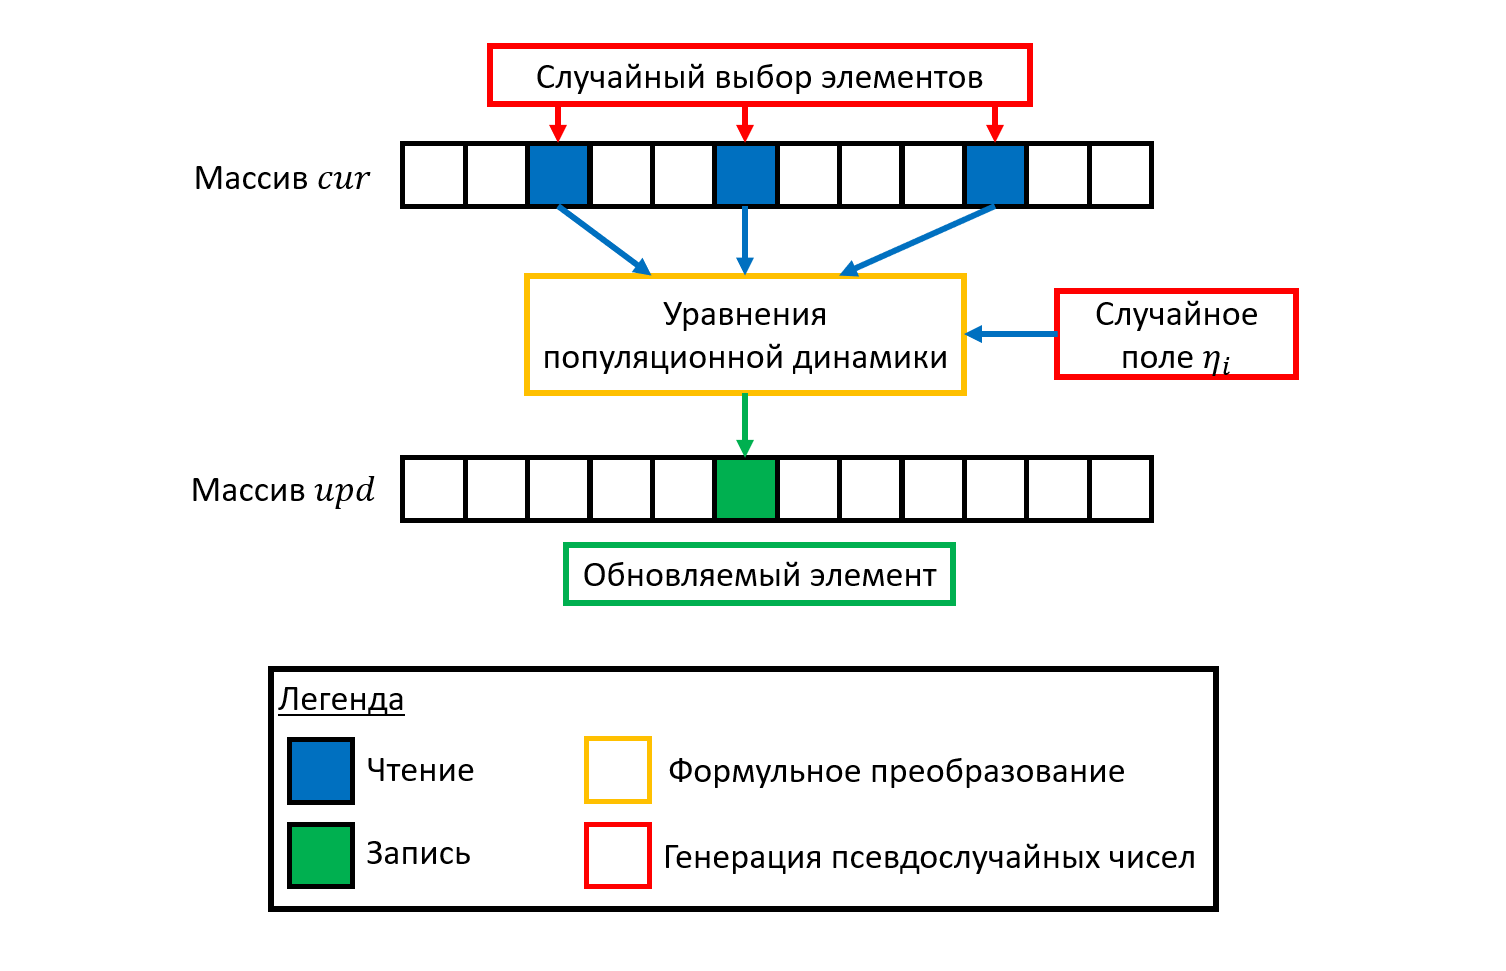
\includegraphics[width=0.8\textwidth]{Convetional_population_dynamics_scheme.png}
	\caption{Принципиальная схема одного шага алгоритма популяционной динамики.}
\end{figure}

\subsubsection{Вопросы сходимости алгоритма}
У алгоритма есть два набора параметров:
\begin{enumerate}
	\item внешние параметры (физические): $\Delta$, $g$, $K$
	\item Внутренние параметры алгоритма: размеры массивов $M$, число итераций $N$, значение параметра уширения уровней $\gamma$. 
\end{enumerate}
Как уже обсуждалось ранее в теоретическом описании алгоритма, физическая ситуация соответствует взятию пределов в следующем порядке:
$$
\lim_{\gamma \rightarrow +0} \lim_{M \rightarrow \infty} \lim_{N \rightarrow \infty}
$$
так что величина $M$ имеют роль схожую с тем, которую в исходной задаче выполняло число узлов графа. Однако, на практике взятие этих пределов сводится к надежде, что начиная с некоторого момента получаемые распределения перестают видимым образом зависеть от этих внутренних параметров. Иными словами, эти пределы берутся только численно, так что полная процедура сводится к следующему
\begin{enumerate}
	\item При фиксированных $\gamma, M$ провести достаточное большое число итераций алгоритм $N^*$, чтобы эмпирическое распределение $P[\gamma, M ,N](G_{i \rightarrow j})$ перестало видимым образом изменяться. Это можно фиксировать, например, по динамике моментов распределения (которые легко поддерживать), а также различными статистическими критериями, вроде Критерия Колмогорова-Смирнова. Оценка на минимальное число необходимых итераций имеет вид $N^{*} \gtrsim \frac{\ln M}{\ln K}$.
	\item Далее, при заданном $\gamma$ ровно тем же способом находится значение $M^*$, после которого распределение $P[\gamma, M, N^*(\gamma, M)]$ перестаёт изменяться. Трудности состоят в том, что оценка на необходимую величину размера выборки в случае делокализованной фазы является очень быстро растущей с уменьшением $\gamma$: $\ln M^{*} \gtrsim \ln K \ln \frac{1}{\gamma}$. 
	Отметим, что полученная оценка получается очень быстро растущей с $\gamma$, что в общем случае усложняет интерпретацию результатов, требуя тщательного анализа данных на предмет насыщения по данным пределам.
	\item Наконец, точно также подбирается параметр $\gamma^*$, характеризующий сходимость численного приближения к истинному распределению $$P\left[ \gamma^*, M^*(\gamma^*), N^*\left( \gamma^*, M^{*}(\gamma^*) \right) \right]$$. Отметим, однако, что для некоторых величин зависимость от регуляризации $\gamma$ будет присутствовать на любых масштабах. В таких случаях требуется изучать факт выхода этих зависимостей на их асимптотическую форму. Примером является величина IPR \eqref{eq:IPR_through_GF}: в зависимости от устройства состояний она будет вести себя или как $L \propto \gamma$ (делокализованная фаза) или выходить на некоторое постоянное значение (соответствует локализации). Разумеется, трудность представляет установления того или иного поведения при анализе данных численного счёта. Далее мы проиллюстрируем практический критерий, по которому будем определять насыщение по данному параметру.
\end{enumerate}
Детали и тонкости практической реализации этой сходимости мы проиллюстрируем далее.  


\subsection{Оптимизация}
Автором данной работы также предлагается оптимизация описанного алгоритма, заключающаяся в том, чтобы не различать обновляемые и текущий массивы. Иными словами, в памяти держится только один массив, который служит и источником для случайного выбор элементов, и местом записи результата вычислений по уравнениям популяционной динамики \eqref{eq:Population_dynamics_final_equations}. Наглядным образом эта модификация представлена в виде схемы на Рис. \ref{fig:Optimized_PD_scheme}.
\begin{figure}[h]
	\label{fig:Optimized_PD_scheme}
	\centering
	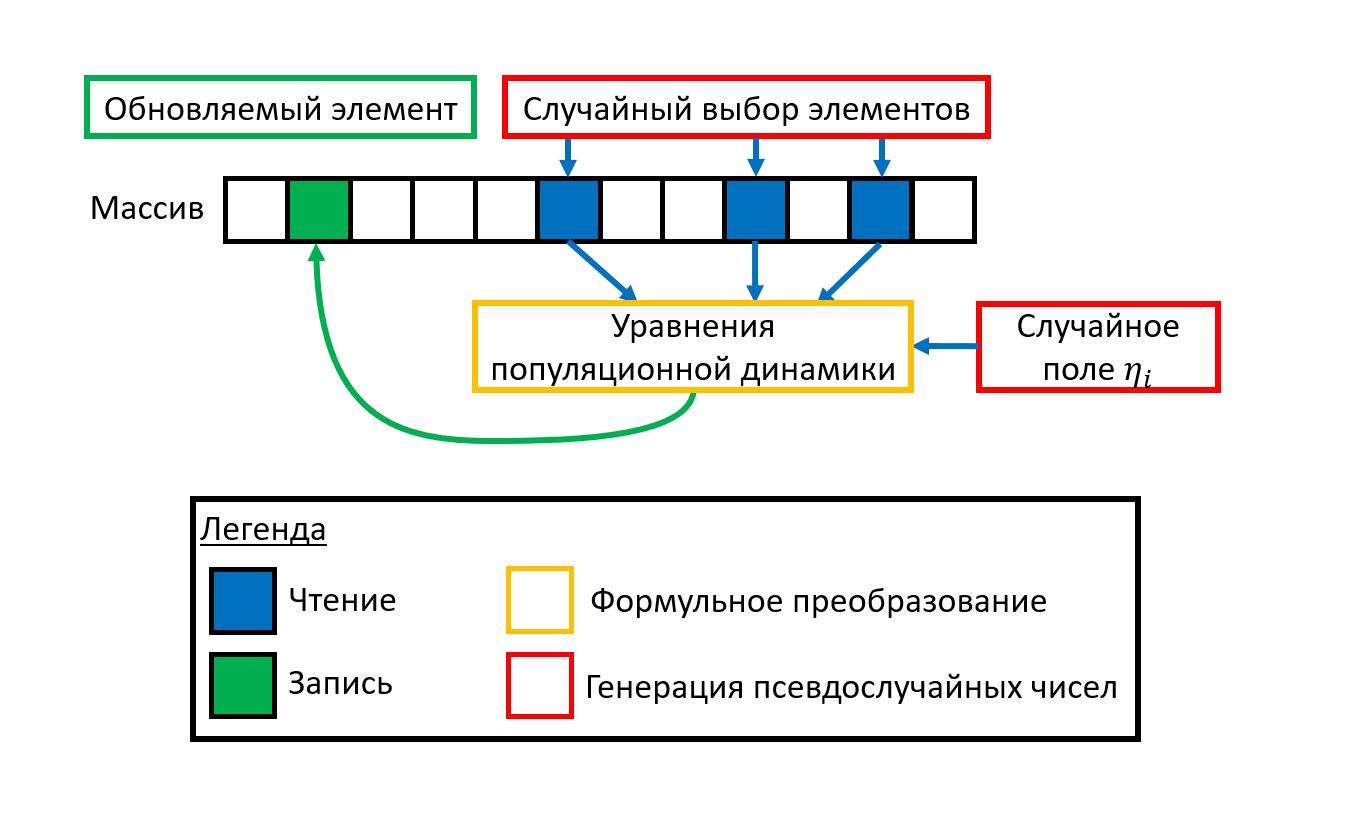
\includegraphics[width=0.8\textwidth]{Optimized_population_dynamics_scheme.png}
	\caption{Принципиальная схема одного шага оптимизированного алгоритма популяционной динамики. Следует сравнивать с Рис. \ref{fig:Population_dynamics_algorythm_scheme}: разница состоит в объединении ролей массивов $cur$ и $upd$}
\end{figure} 

Целями этой оптимизации является
\begin{itemize}
	\item очевидная экономия памяти, которая необходима для достижения упомянутой сходимости по размеру выборки $M$, так как характерные значения $M \sim 10^8$ лежат на границе доступных для вычислений ресурсов
	\item Гораздо менее очевидная оптимизация по количеству необходимого для сходимости количества итераций $N$. Строгих доводов о том, почему оптимизированный вариант алгоритма должен работать быстрее, нету, однако качественно получаемое на практике ускорение можно объяснить тем, что при подходе к концу массива в рамках одной итерации массив уже эффективно содержит обновлённую выборку, поэтому при генерации нового значения элементы из конца массива будут с большей вероятностью воспроизводить результат работы на большем количестве итераций. Тем самым, за одну итерацию этот алгоритм эффективно совершает несколько итераций классического варианта.
\end{itemize} 

Отметим, тем не менее, что строго говоря, существует вопрос о степени правильности получаемый выборки, поскольку, как отмечено выше, конец массива эффективно претерпел большее число итераций, нежели его начало. Однако, поскольку мы занимаемся поиском \textit{стационарной точки} отображения \eqref{eq:Population_dynamics_final_equations}, то на поздних этапах распределение эффективно <<забывает>> количество сделанных итераций, а потому результаты работы обоих алгоритмов (классического и оптимизированного) идентичны. Разумеется, данные рассуждения являются сугубо качественными, и серьёзным аргументом будет лишь практическая проверка степени схожести ответов для двух версий алгоритма.



\section{Тестирование и интерпретация особенностей работы алгоритма}
В этом разделе будут обсуждены основные практические аспекты применения описанного выше алгоритма популяционной динамики. При обсуждении рассматриваться будет только поведение локальной плотности состояний, как более наглядной величины для демонстрации ключевых особенностей.

\subsection{Эффективность использованных оптимизаций}
Прежде всего, проверим, является ли предложенная оптимизированная версия алгоритма рабочей. Критерием идентичности алгоритмов служит идентичность распределений плотности после выхода в стационарный режим. Детали проверки следующие:
\begin{itemize}
	\item на каждой итерации записывалась полная выборка, из которой потом вычислялись все нужные характеристики распределения.
	\item Параметры симуляций выбирались так, чтобы наблюдалось наиболее широкое распределение $\rho$, что даёт больше возможностей для явления потенциальных различий в алгоритмах. Численные значения следующие:
		\begin{itemize}
			\item Внешние физические параметры: $ K = 2, g = 0.15, \Delta = 2\exp \left\{ - \frac{1}{g} \right\}$
			\item Постоянные параметры алгоритма: $ \gamma = 10^{-7}, M = 2^{22} \approx 4.2 \cdot 10^6$
			\item Полное число итераций $N = 256$.
		\end{itemize}
	\item Стационарное значение оценивалось усреднением по большому числу итераций в области видимого постоянства значения. В данном случае, это диапазон  $N \in [60, 256]$.
\end{itemize}
Сравнение получающихся распределений приведено на Рис. \ref{fig:Methods_comparison_stationary_distribtution}, а демонстрация скорости сходимости на примере первых моментов приведена на Рис. \ref{fig:Methods_comparison_moments_convergence}.
\begin{figure}[h]
	\label{fig:Methods_comparison_stationary_distribtution}
	\centering
	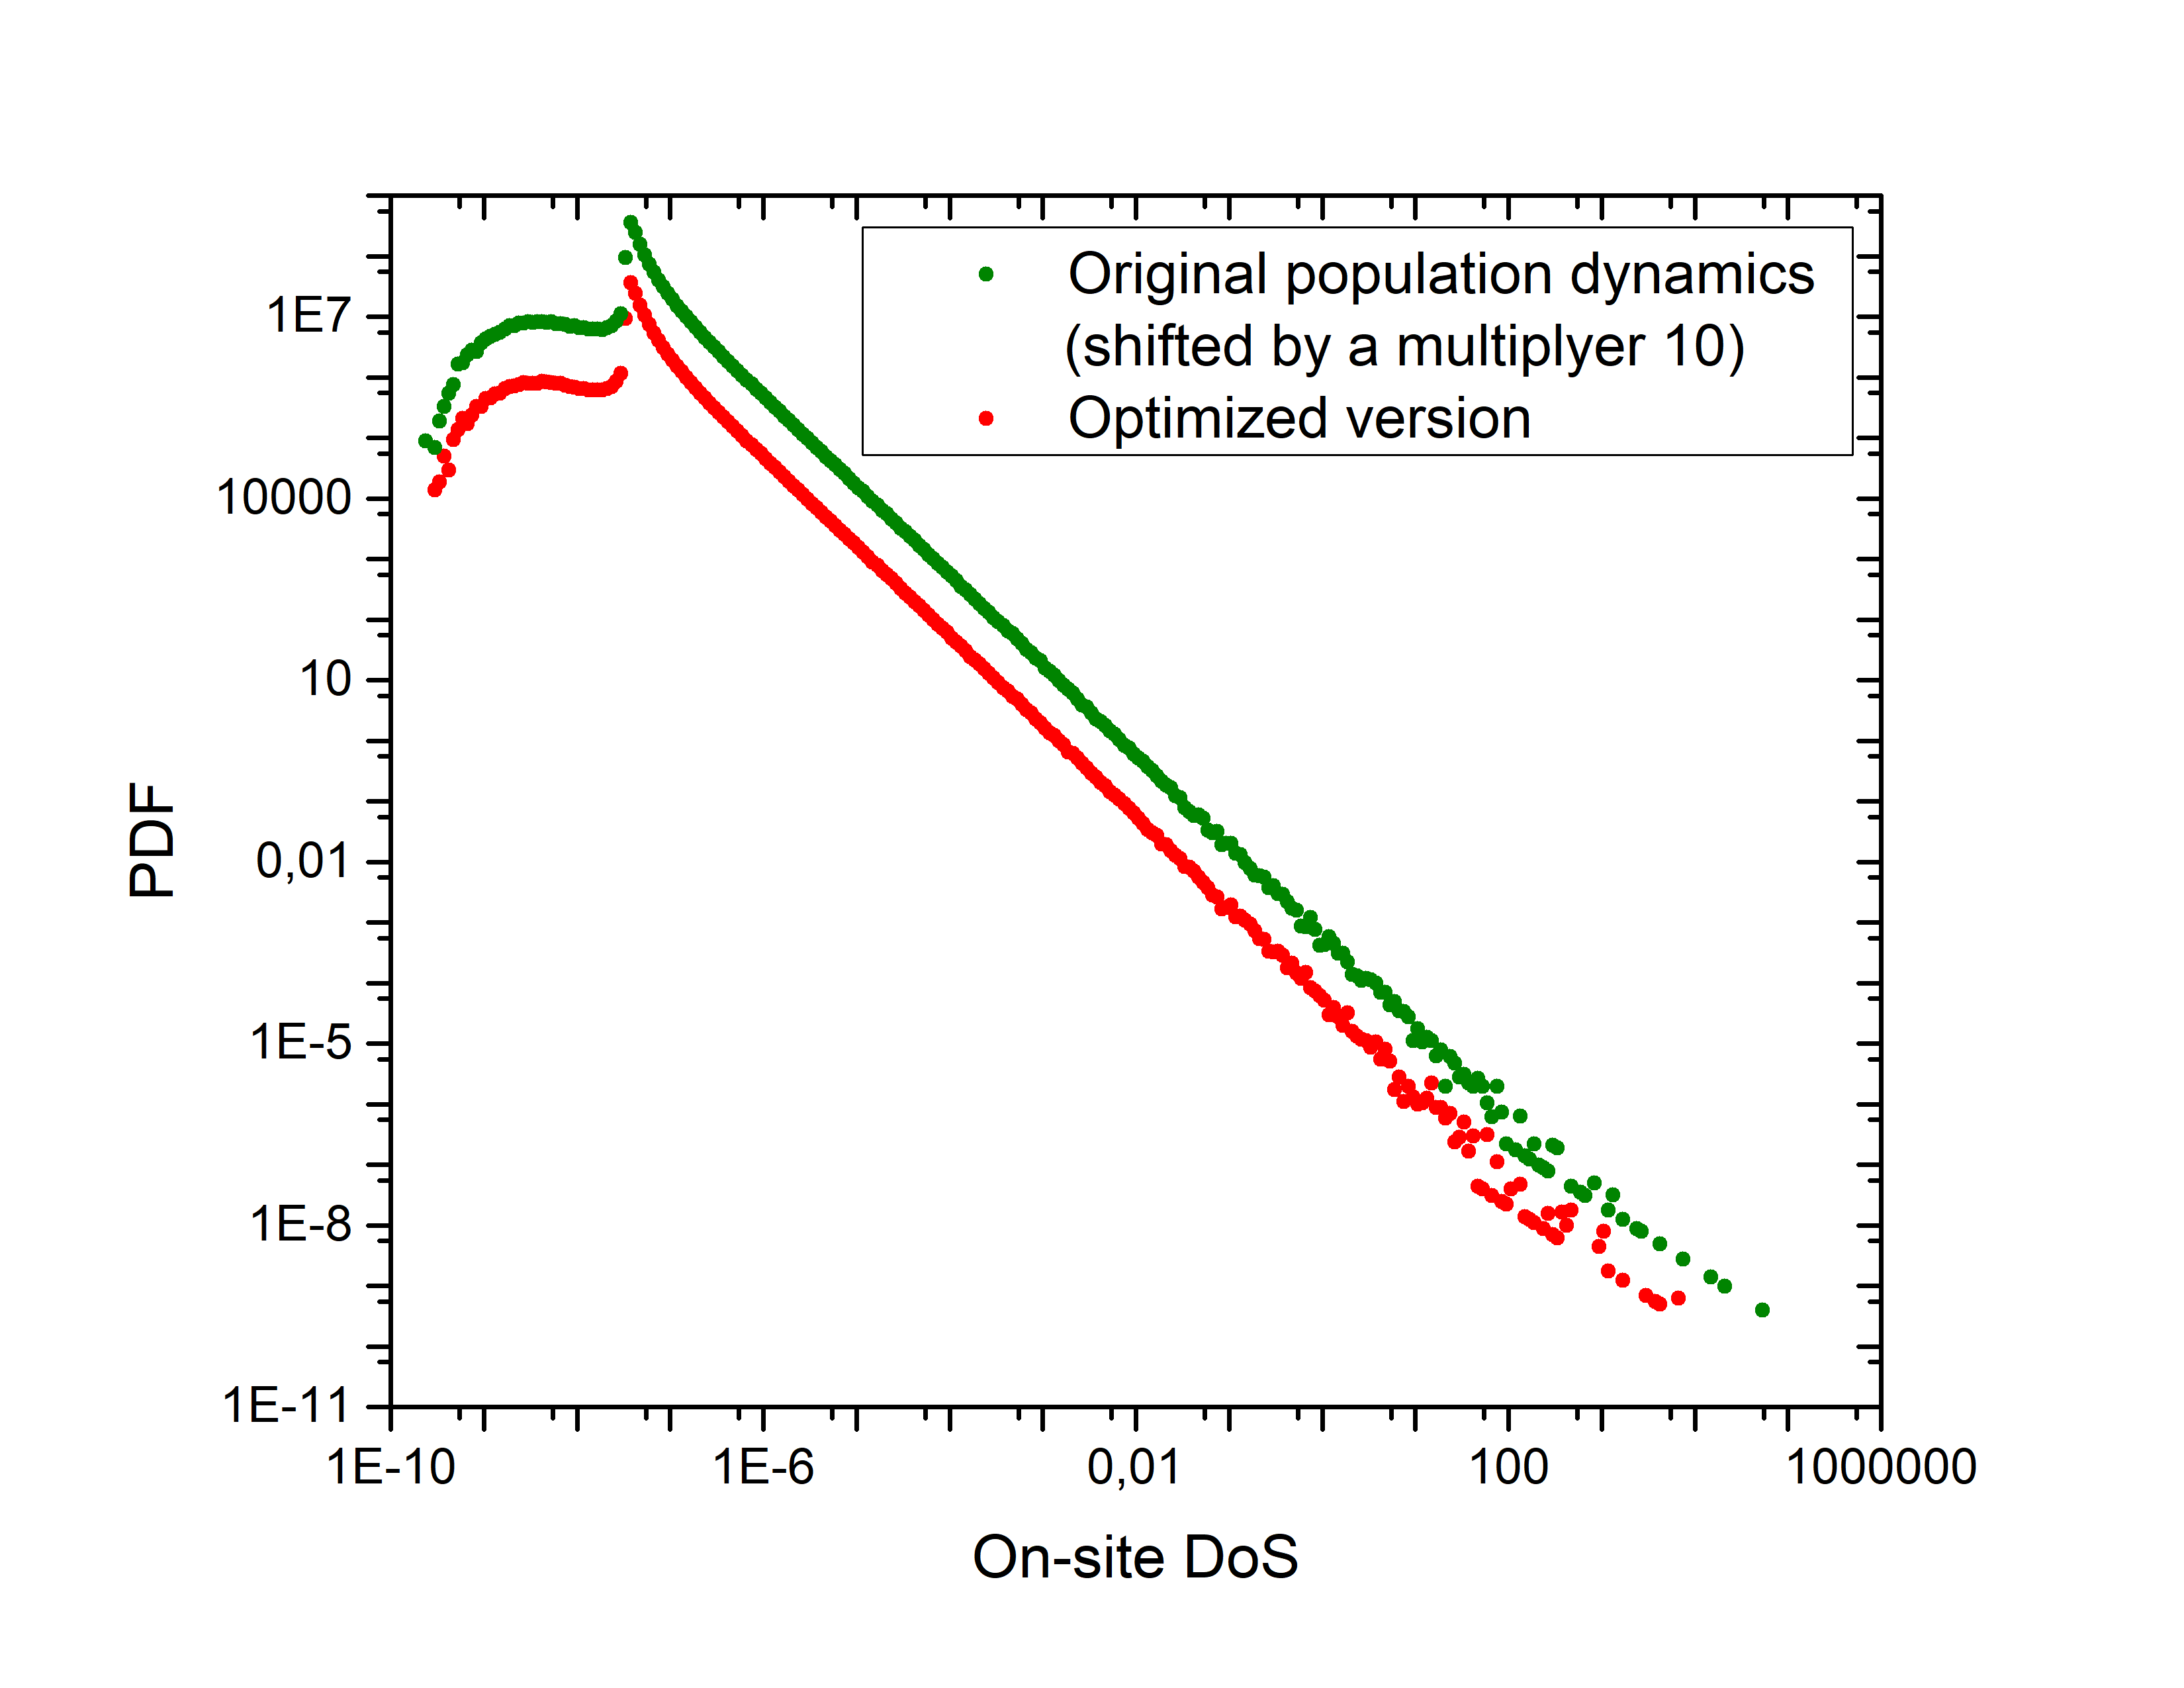
\includegraphics[width=0.8\textwidth]{Algo_comp_versions_distr.png}
	\caption{Стационарное ($N = 128$) эмпирическое распределение плотности для обеих версий, причём данные для наглядности сдвинуты постоянным множителем $10$, так как при наложении они совпадают (очевидно, постоянный множитель портит только нормированность распределения, но не его форму). Подробные технические данные симуляции см. в тексте.}
\end{figure}

\begin{figure}[h!]
	\label{fig:Methods_comparison_moments_convergence}
	\centering
	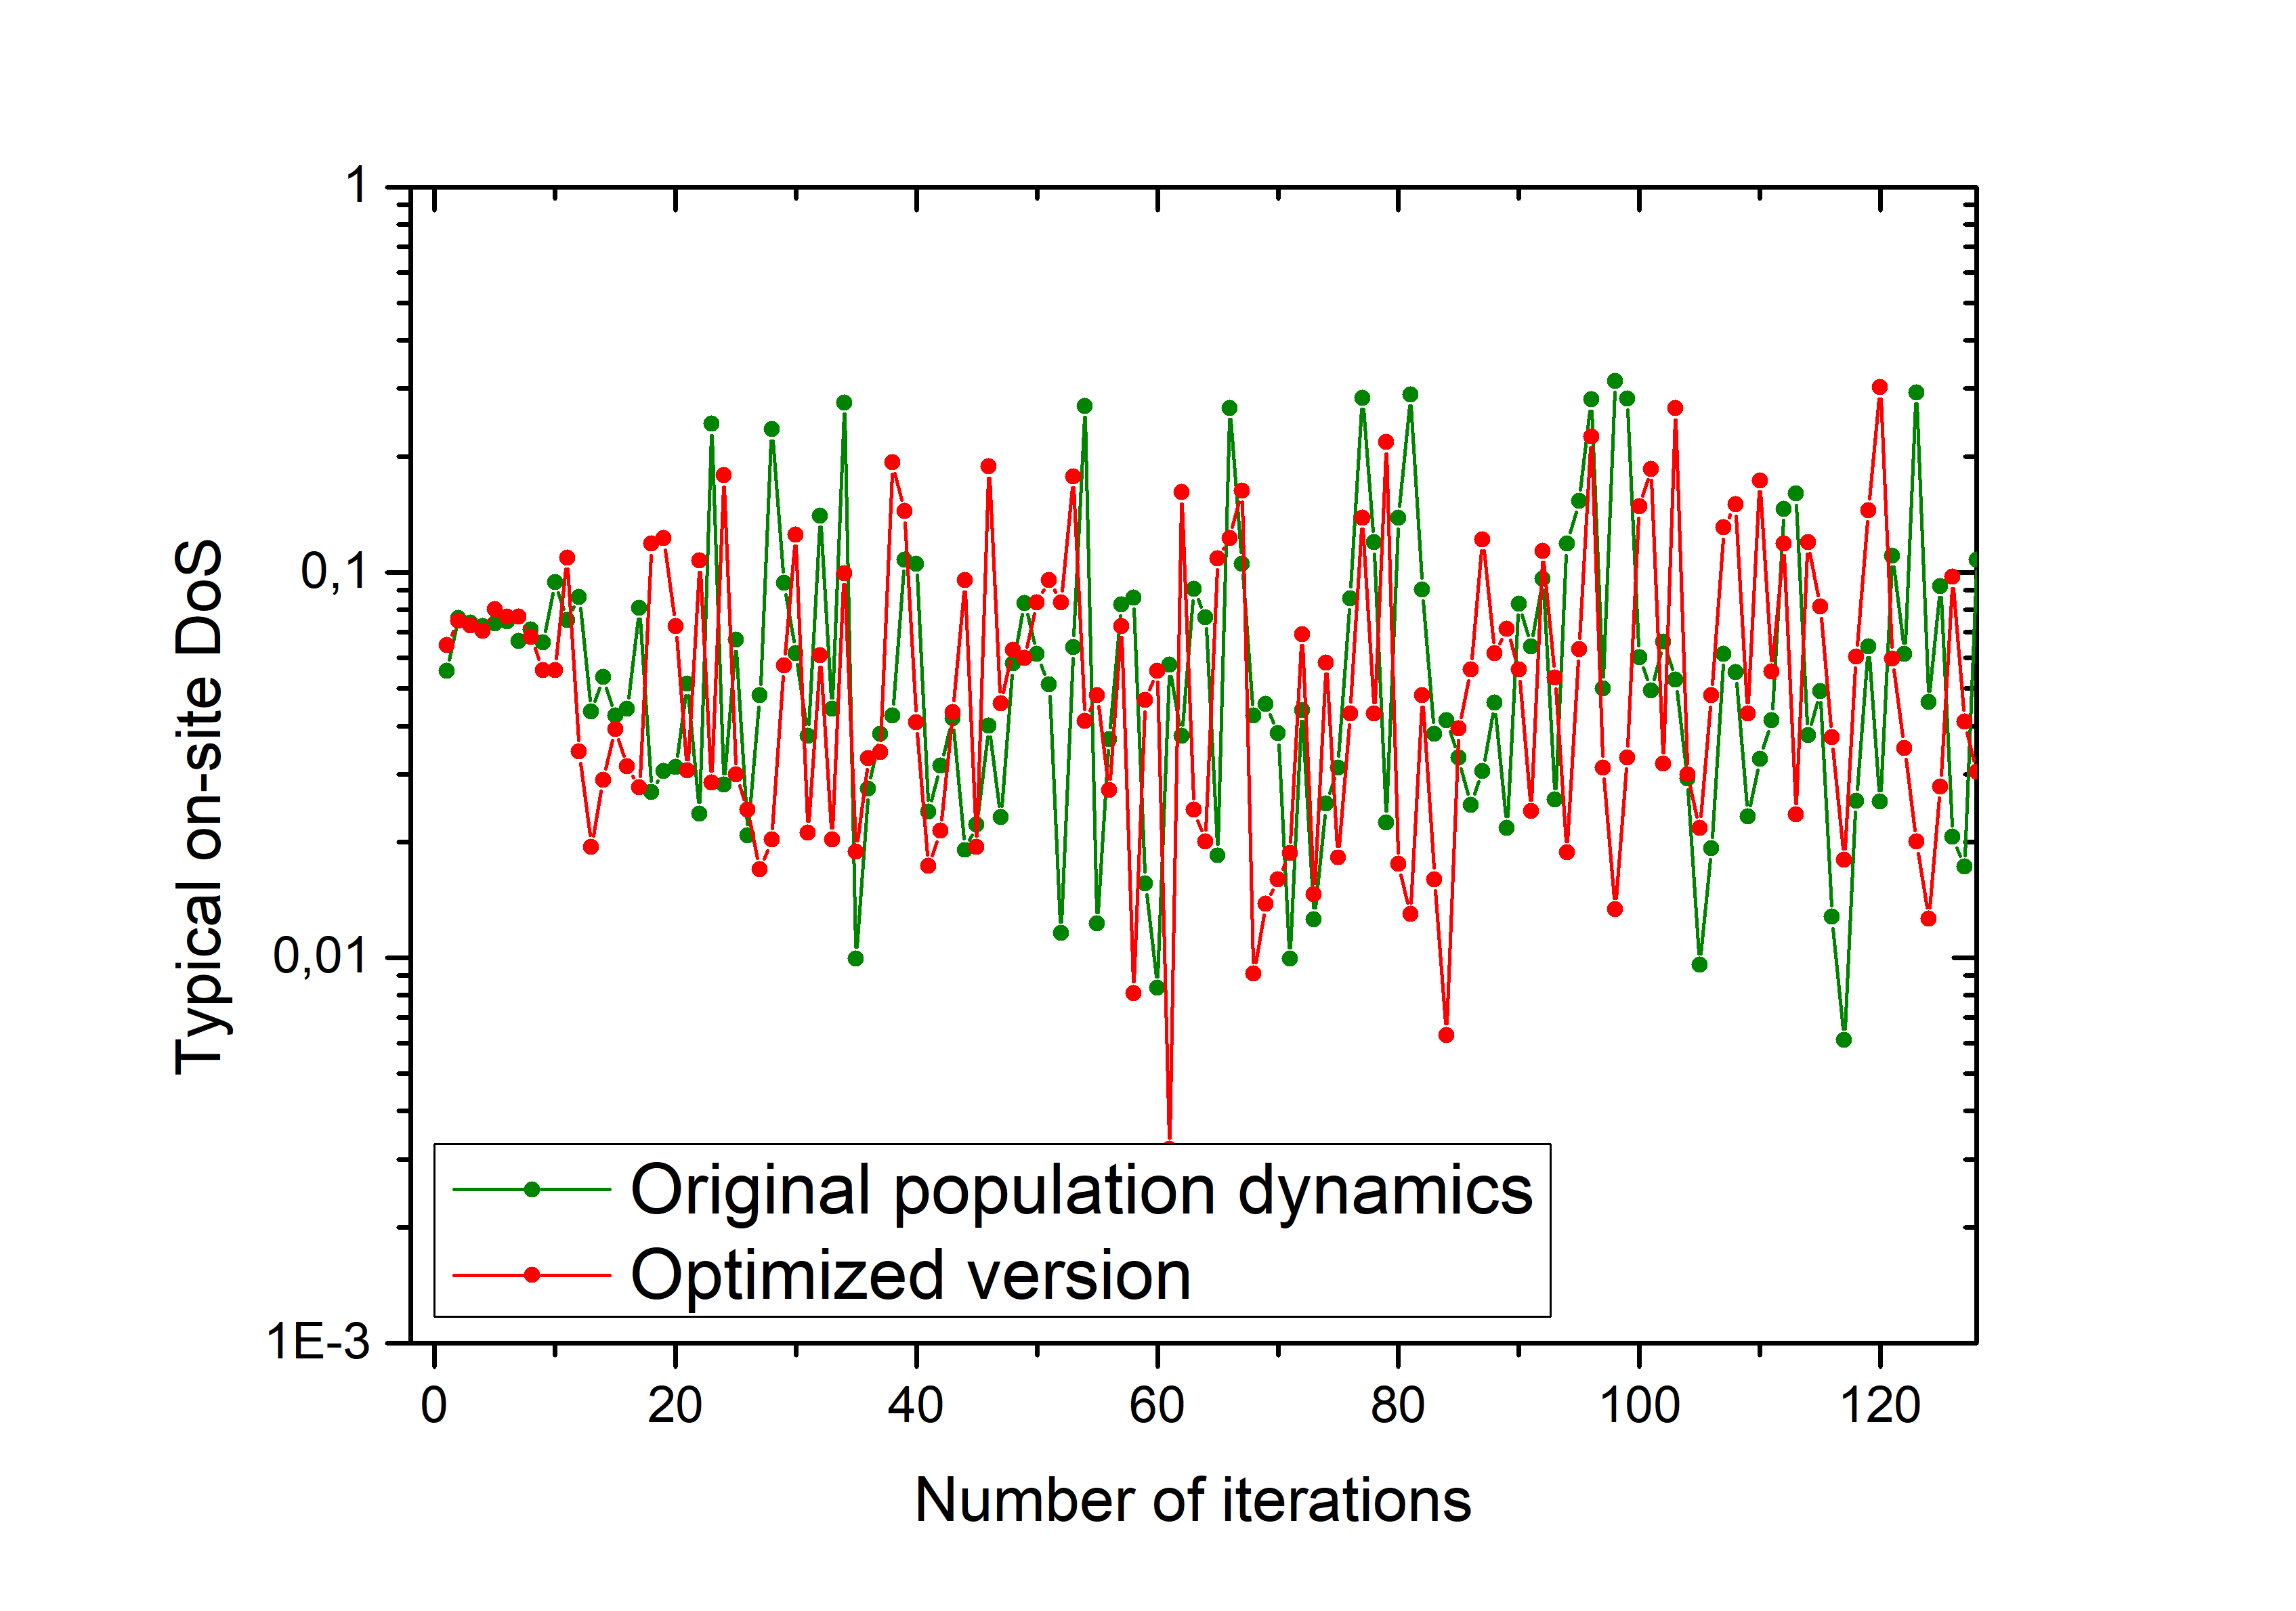
\includegraphics[width=0.49\textwidth]{Algo_comp_versions_mean.png}
	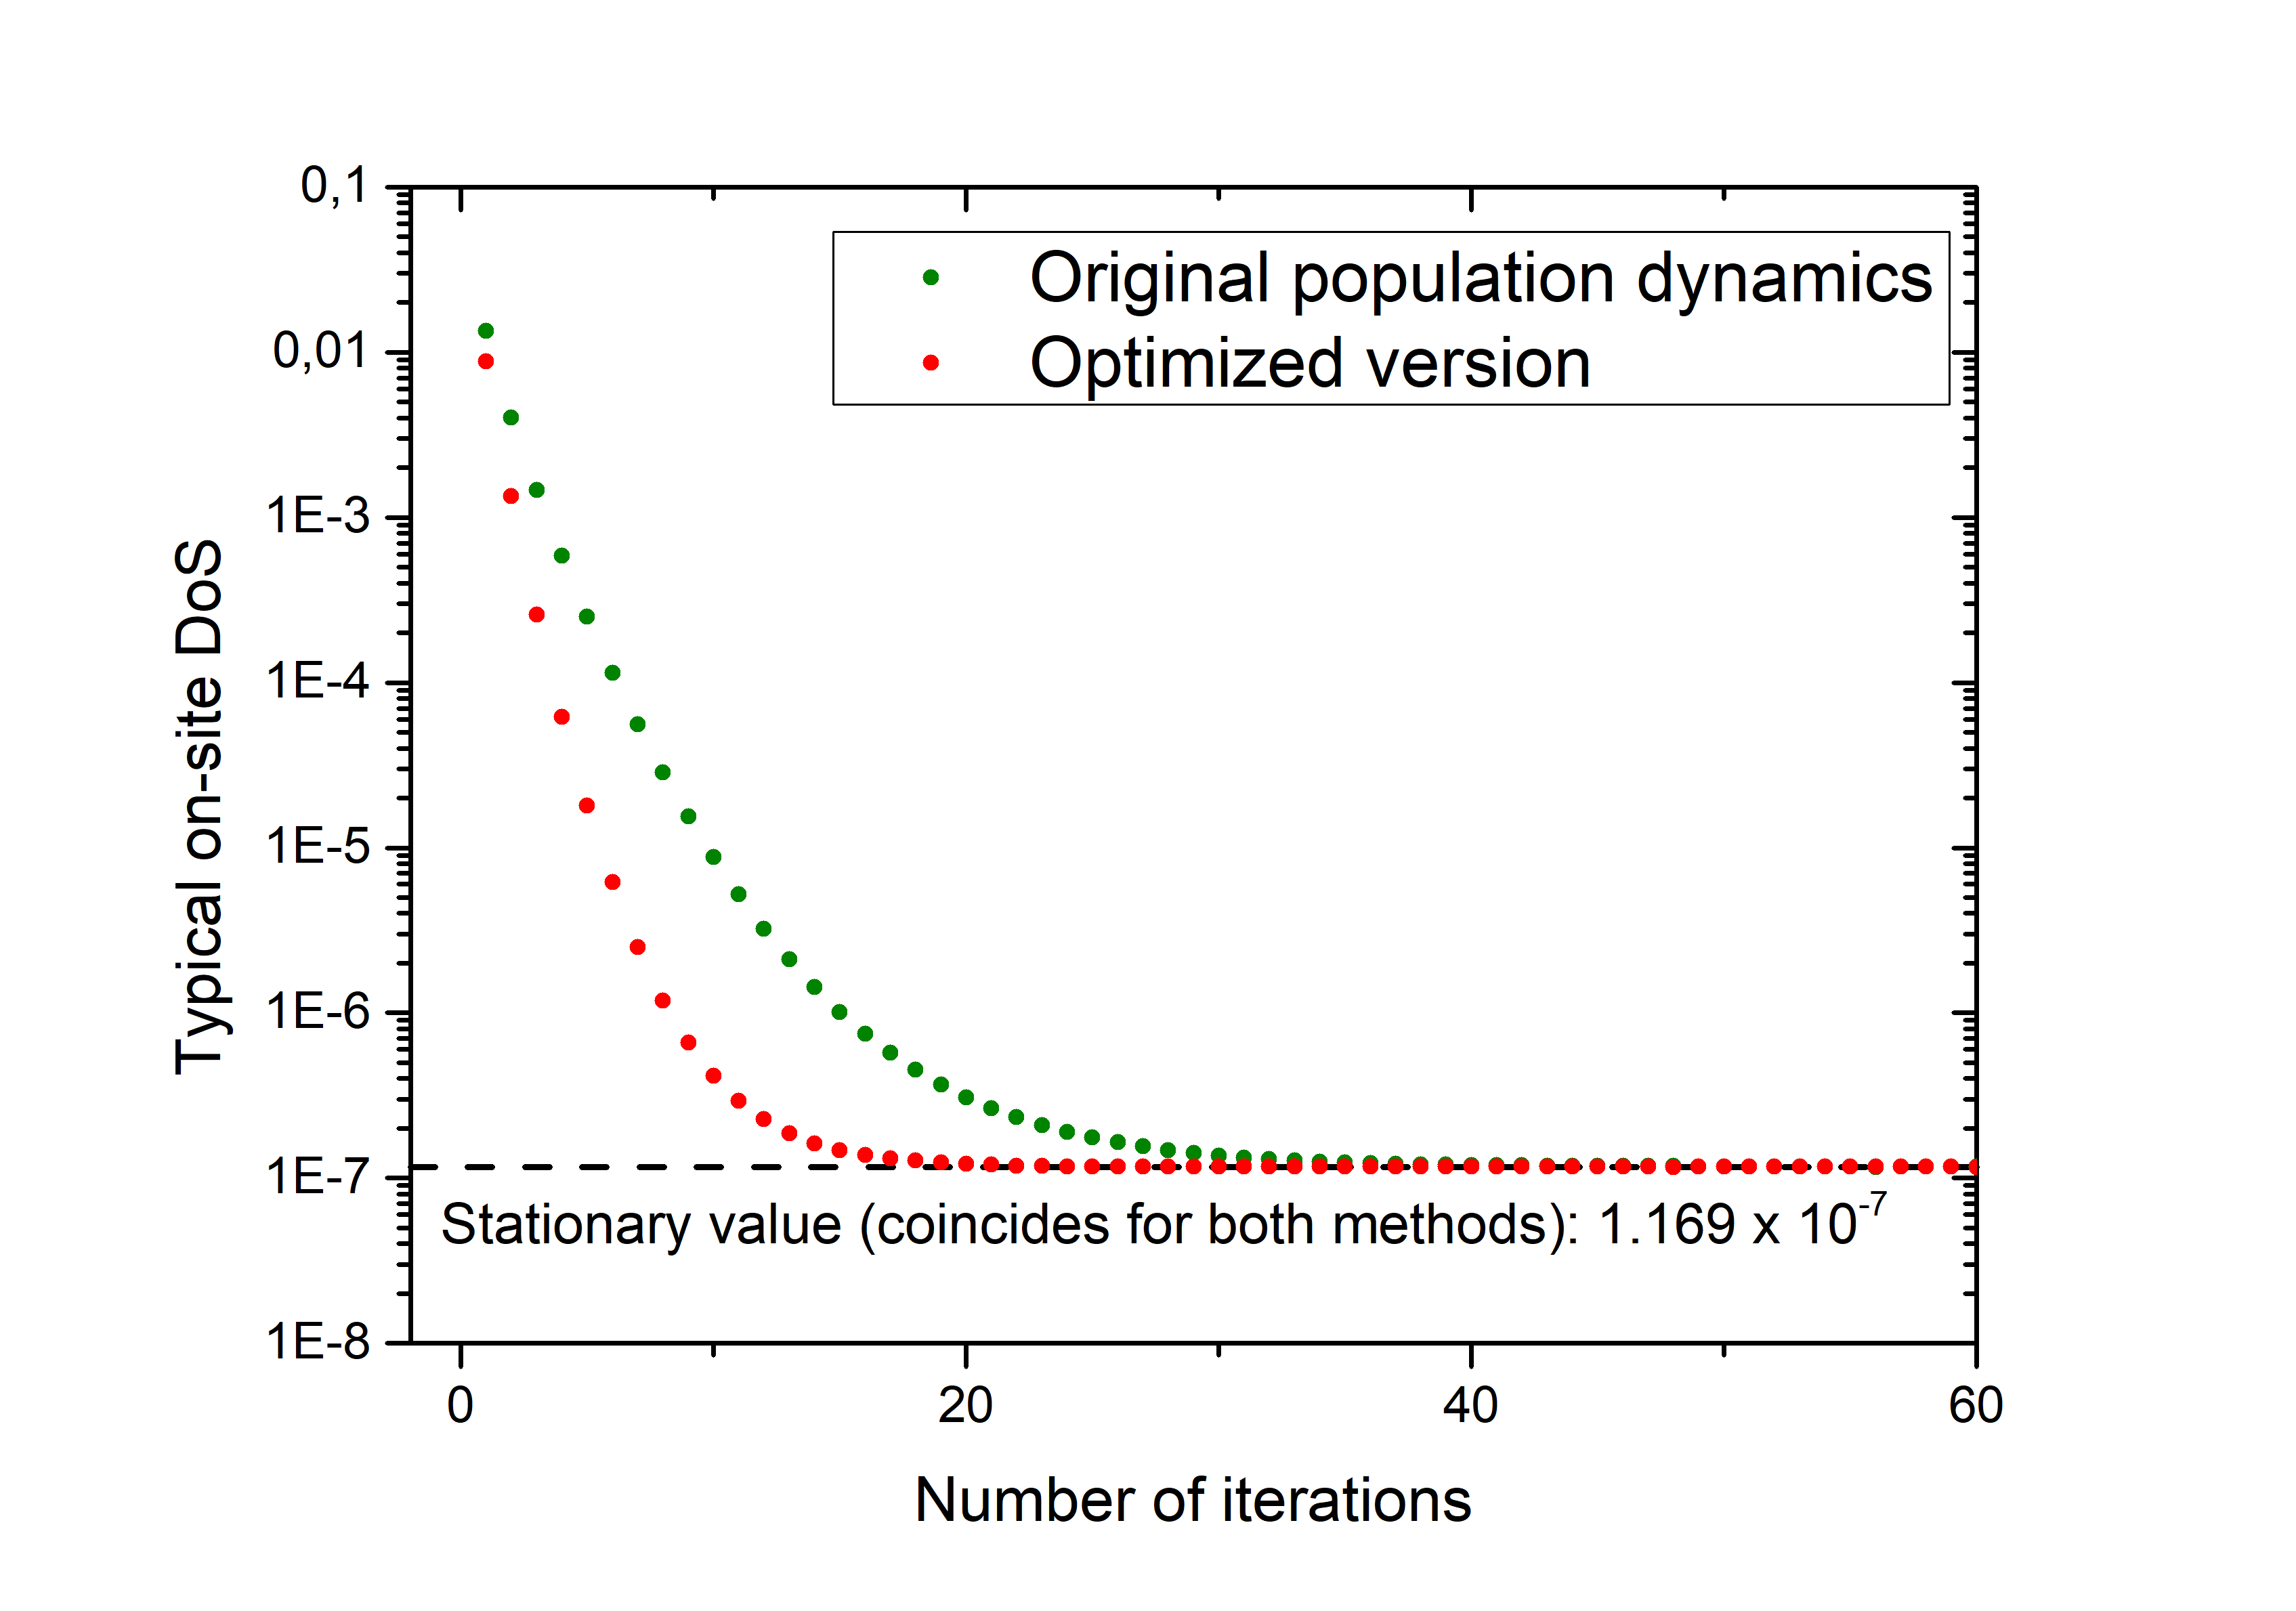
\includegraphics[width=0.49\textwidth]{Algo_comp_versions_typical.png}
	\caption{Слева: зависимость средней плотности состояний $\langle \rho \rangle$ от числа итераций для обеих версий. Справа: зависимость типичной плотности состояний $\exp{\langle \ln \rho \rangle}$ от числа итераций для обеих версий. Подробные технические данные симуляции см. в тексте.}
\end{figure}

Обзор специфики формы распределения см. в \autoref{Result}, а на данный момент основные выводы по данным следующие:
\begin{itemize}
	\item как наглядно видно из Рис. \ref{fig:Methods_comparison_stationary_distribtution}, алгоритмы дают абсолютно идентичные результаты, так как формы графиков полностью одинаковые, а при наложении они тождественно совпадают.
	\item Как показывают данные для зависимости типичной плотности состояний от числа итераций на Рис. \ref{fig:Methods_comparison_moments_convergence} слева, оптимизированная версия работает примерно в два раза быстрее, что для неигрушечных симуляций сэкономило автору работы недели компьютерного времени.
	\item Данные по средней плотности состояний на Рис. \ref{fig:Methods_comparison_moments_convergence} справа говорят о том, что оба метода в одинаковой степени чувствительны к статистическим флуктуациям, обусловленным конечным размером выборки (об этом подробнее см. далее).
\end{itemize}
Как итог, можно утверждать, что оптимизация явно имеет ощутимый смысл.


\subsection{Сравнение с точной диагонализацией}
Для проверки общей валидности применяемого метода предлагается сравнить его с процедурой \textit{точной диагонализации}, гарантированно воспроизводящей правильное распределение плотности состояний для конечных системы. Суть этой процедуры кратко описывается следующим образом:
\begin{enumerate}
	\item генерируется случайный $K$-регулярный граф некоторого размера $M \sim 10^3$.
	\item Генерируется случайный набор полей $\eta_i$, и по определению \eqref{eq:Local_operator_definition} составляется матрица $C$. 
	\item Применяется численный алгоритм <<FEAST>> поиска всех собственных векторов матрицы с собственным числом, лежащим в конечной малой окрестности $\delta E$ требуемого собственного числа ($1$ в нашем случае).
	\item Локальная плотность состояний на каждом узле оценивается по формуле
	$$
	\rho_i = \frac{1}{\delta E} \sum_k \left| \left\langle \psi_k | i \right\rangle \right|^2
	$$
	где $\psi_k$ -- найденные вектора, $i$ -- номер узла.
	\item По значениям найденных плотностей в нескольких реализациях беспорядка составляется выборка.
\end{enumerate}

\begin{figure}[h!]
	\label{fig:Exact_digonalization_different_matrix_sizes}
	\centering
	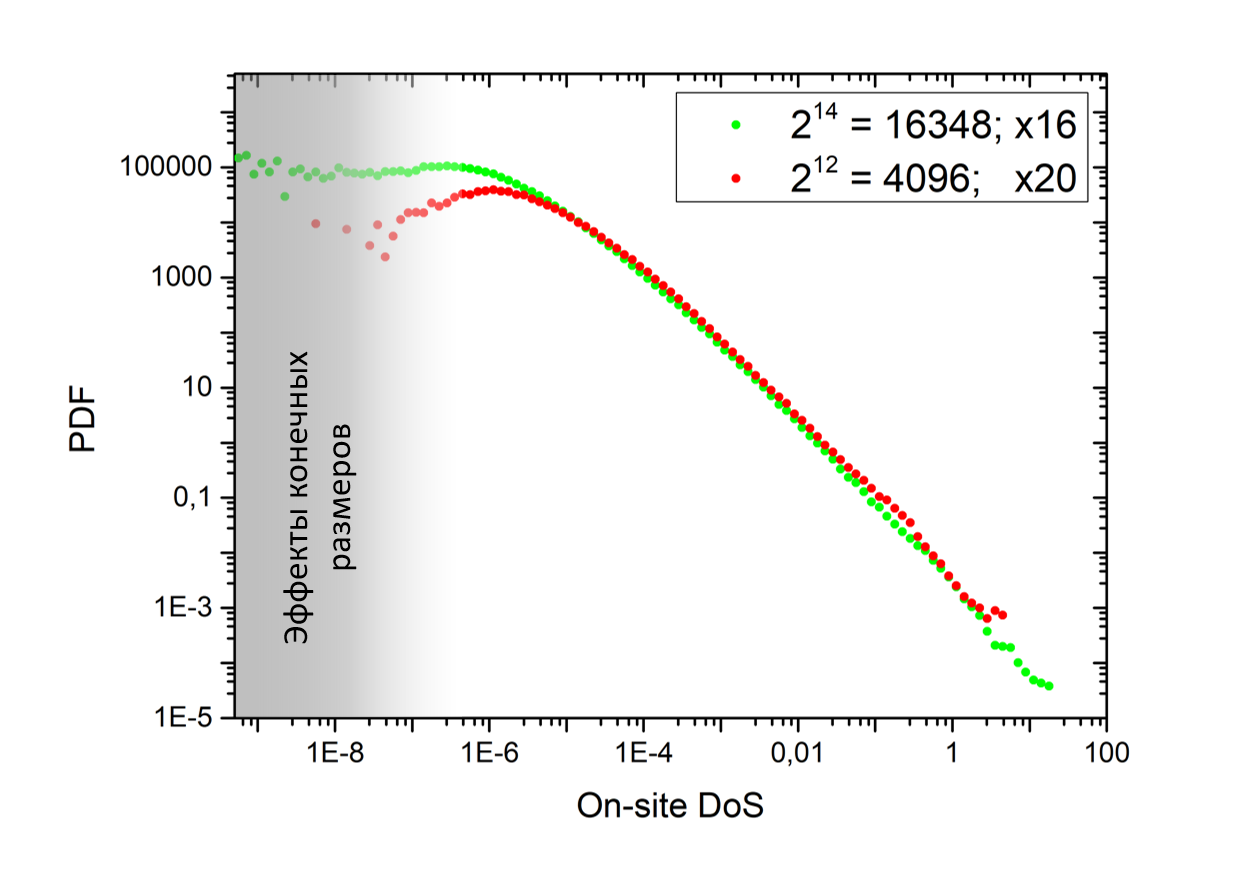
\includegraphics[width=0.8\textwidth]{ED_different_sizes_comp_distr.png}
	\caption{Эмпирическое распределение плотности состояний, полученное методом точной диагонализации для двух различных размеров матриц: 16 реализаций системы с $2^{14} = 16348$ узлами и 20 реализаций системы с $2^{12} = 4096$ узлами. Ширина окна по энергии $\delta E$ подстраивалась так, чтобы плотность состояний оценивалась по примерно одному и тому же количеству найденных состояний независимо от размера системы. Серым выделена область, в которой заметны существенные различия между данными из-за эффектов конечных размеров.}
\end{figure}

Особенности реализации и детали получения физически правильных результатов этой процедурой мы здесь обсуждать не будем. Продемонстрируем лишь тот факт, что полученная выборка, как и ожидается от такой этого метода, сильно чувствительна к размеру системы: данные для двух различных размеров матриц показаны на Рис. \ref{fig:Exact_digonalization_different_matrix_sizes}. Как видно из этих результатов, чтобы аккуратно исследовать термодинамический предел, необходимы гораздо большие размеры матриц, однако сложность $O(M^2)$ и такая же асимптотика для объёма занимаемой памяти делают этот метод малопригодным для наших целей.

\begin{figure}[h!]
	\label{fig:Comparison_PD_vs_ED}
	\centering
	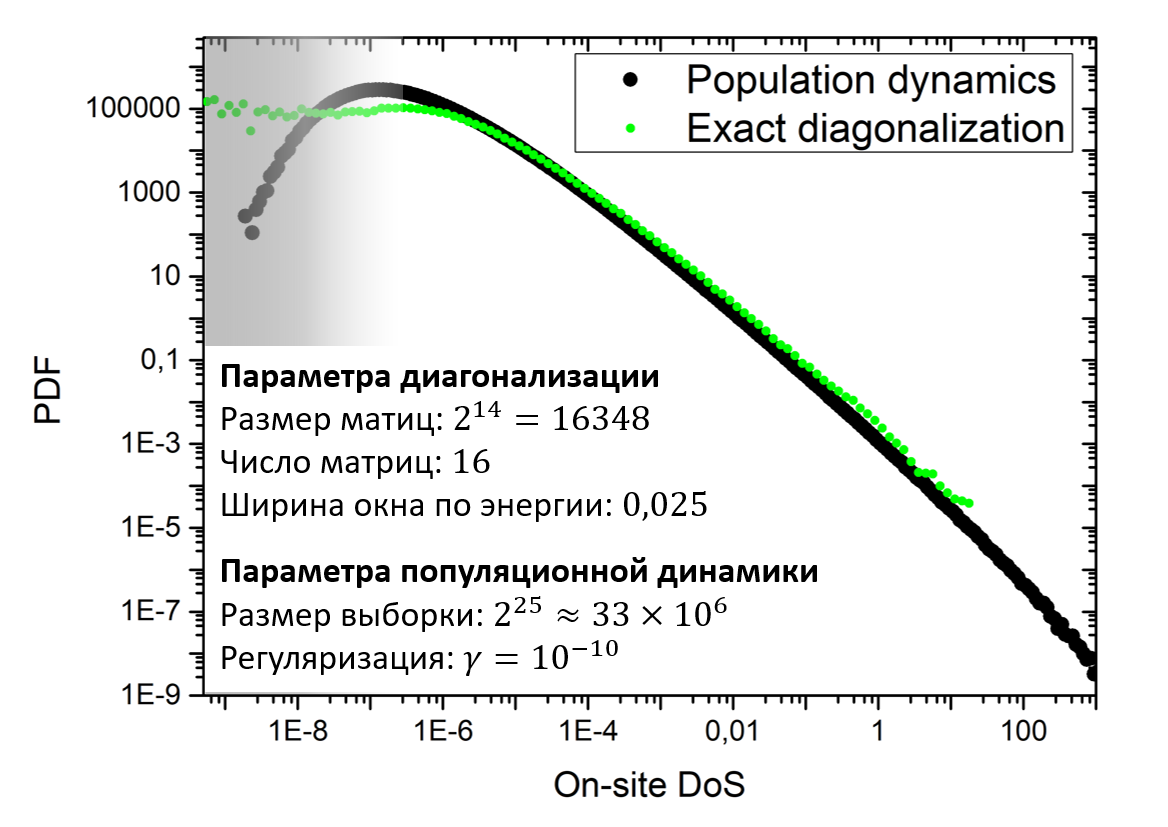
\includegraphics[width=0.8\textwidth]{Comparison_ED_vs_PD.png}
	\caption{Сравнение эмпирического распределения плотности состояний, полученных методами популяционной динамики и точной диагонализации. Значения внутренних параметров каждого из алгоритмов подписаны на рисунке. Серым отмечена область, не являющаяся достоверной для алгоритма точной диагонализации из-за эффектов конечных размеров.}
\end{figure}

Сравним данный <<эталонный>> метод с методом популяционной динамики. Результаты симуляции показаны на Рис. \ref{fig:Comparison_PD_vs_ED}. Значения физических параметров следующие: $ K = 10, g = 0.15 , \Delta = 2 \exp\left\{ -\frac{1}{g} \right\}$. Значения внутренних параметров обоих алгоритмов также указаны на Рис. \ref{fig:Comparison_PD_vs_ED}

Как следует из результатов, наш метод показывает себя полностью состоятельным, а также способным разрешить меньшие значения плотности состояний, реализуемые только в очень больших системах, недоступных для метода точной диагонализации. Отметим также, что авторами было проведено исследование поведения IPR, также идентичное в обоих методах.


\subsection{Особенности поведения численной процедуры при различных внутренних параметрах алгоритма}
В данном разделе мы опишем влияние внутренних параметров алгоритма популяционной динамки на результат его работы, прокомментируем возможные нефизические ситуации, и опишем общие идеи интерпретации данных, получаемых описанной численной процедурой. Существенно, речь далее будет идти о свойствах делокализованных состояний, так как все имеющиеся в распоряжении автора данные демонстрируют только такое поведение. Перечисленные ниже особенности не являются чем-то новым, однако их надо держать в уме при интерпретации данных. Их основной список следующий:
\begin{itemize}
	\item Динамические особенности поведения при итерировании алгоритма:
	\begin{itemize}
		\item хорошо определённое число итераций $N^{*}$, необходимое для установления распределения;
		\item зависимость $N^{*}$ от остальных внутренних параметров алгоритма $M, \gamma$;
		\item сильные флуктуации первых моментов распределения от итерации к итерации даже в стационарном режиме;
		\item хорошо определённое, слабо флуктуирующее значение типичного.
	\end{itemize}
	\item Особенности стационарного поведения:
	\begin{itemize}
		\item плохая статистика на верхней и нижней границах распределения при малых размерах выборки;
		\item резкая отсечка, пропорциональная $\gamma$, на нижней границе при недостаточно малых $\gamma$.
		\item В режиме насыщения плотности состояний по $\gamma$ величина IPR практически линейно зависит от $\gamma$, что соответствует физическому поведению $\lim_{\gamma \rightarrow +0} = 0$ и, соответственно, делокализованной фазе.
	\end{itemize}
\end{itemize}

Далее мы продемонстрируем наиболее информативные из указанных особенностей. С учётом вышесказанного, итоговая последовательность действий для корректного применения алгоритма следующая:
\begin{itemize}
	\item при использовании метода необходимо отследить несколько значений типичной плотности состояний при различном числе итераций и убедиться, что они совпадают;
	\item далее, необходимо удостовериться в независимости получаемых ответов от величин $\gamma$, рассмотрев зависимость типичной плотности состояний и IPR от $\gamma$ при нескольких разных значениях $M$: одна из этих величин должна насыщаться некоторым значением, а вторая -- демонстрировать уверенное степенное поведение, и в зависимости от результата делается заключение о структуре состояний (локализация / делокализация) \cite{AAT}.
\end{itemize}

\subsubsection{Влияние внутренних параметров $M, \gamma$ на сходимость по числу итераций $N$}
Прежде всего, продемонстрируем, как зависят средняя и типичная плотность состояний от числа итераций алгоритма, и как на характеристики сходимости влияют оставшиеся два внутренних параметра алгоритма $M, \gamma$. В нашем анализе мы не будем подробно останавливаться на IPR, поскольку его поведение \textit{во всём исследованном диапазоне параметров одинаково}  и имеет вид линейного по $\gamma$ поведения, слабо чувствительного к прочим параметрам. На Рис. \ref{fig:Convergence_for_various_gamma} приведены зависимости средней $\langle \rho \rangle$ и типичной $\exp \langle \ln \rho \rangle$ плотности состояний для различных $\gamma$, а на Рис. \ref{fig:Mean_convergence_for_various_M} --- данные только для среднего с различными небольшими размерами выборки $M$ (вид зависимости для типичного недемонстративен). Фиксированные физические параметры следующие: $K = 2, g = 0.15, \Delta = 2 \exp \left\{ -\frac{1}{g} \right\}$.

\begin{figure}[h!p]
	\label{fig:Convergence_for_various_gamma}
	\centering
	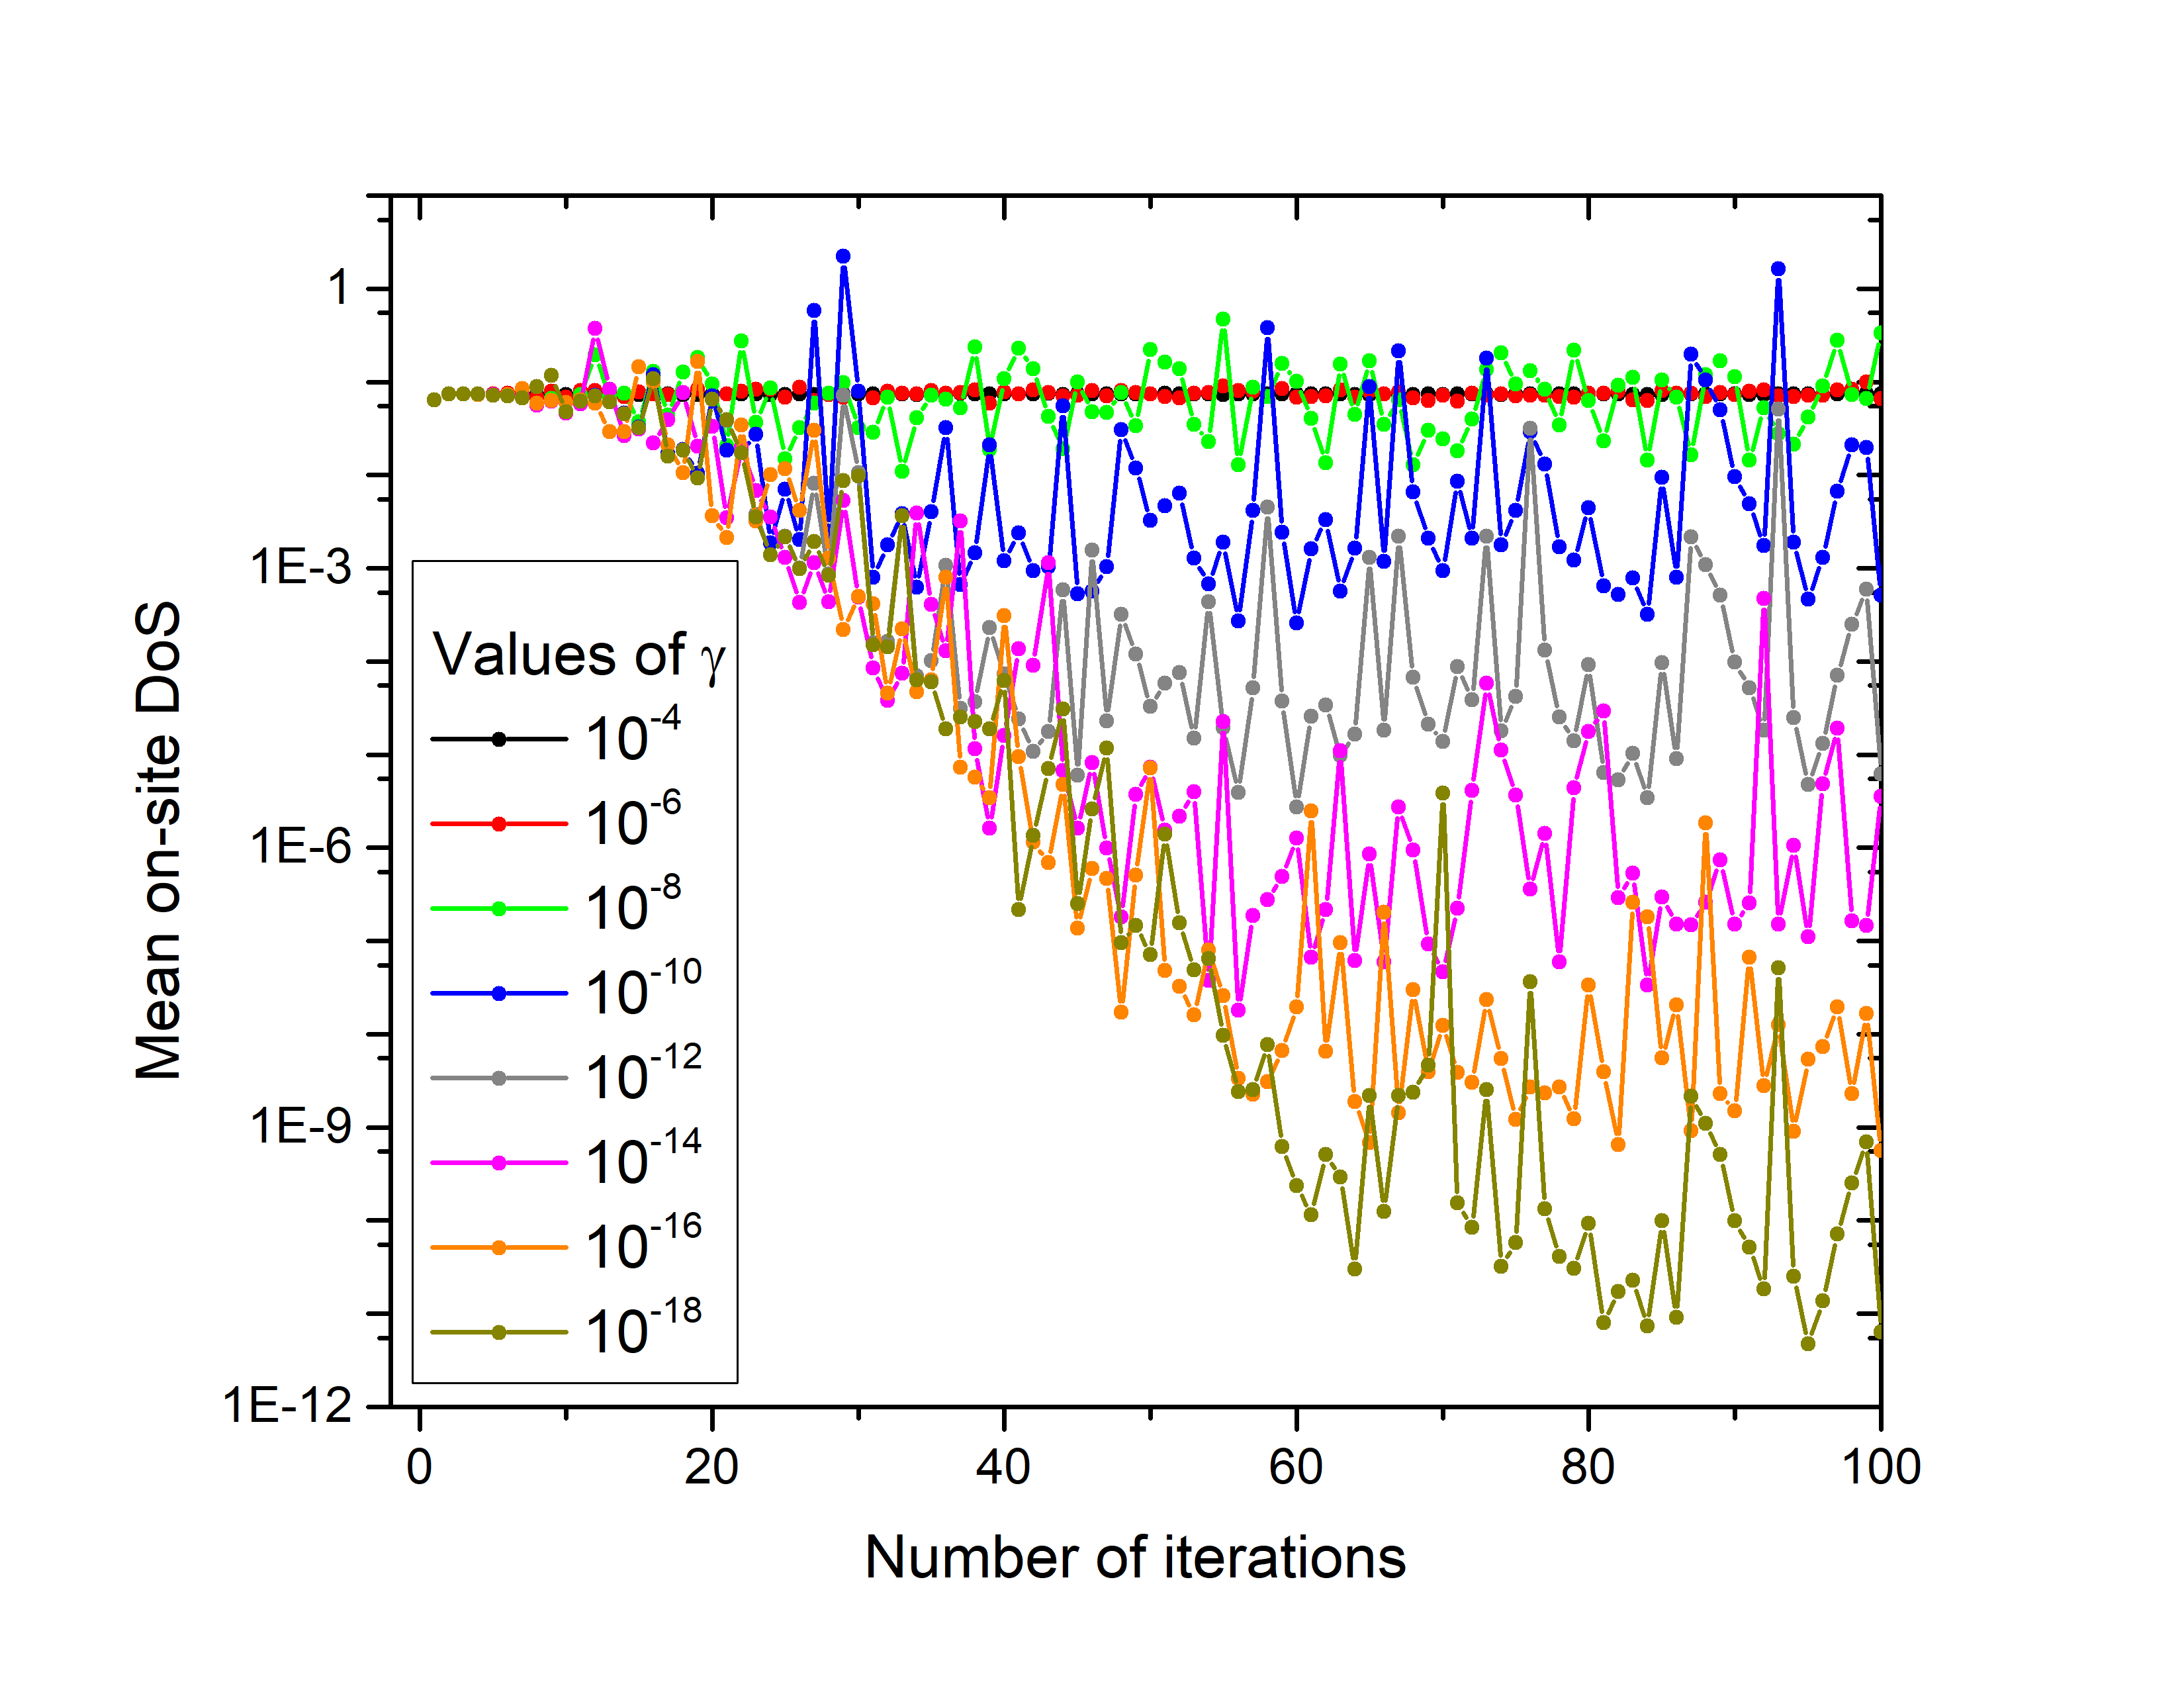
\includegraphics[width=0.85\textwidth]{Mean_convergence_various_gamma.png}
	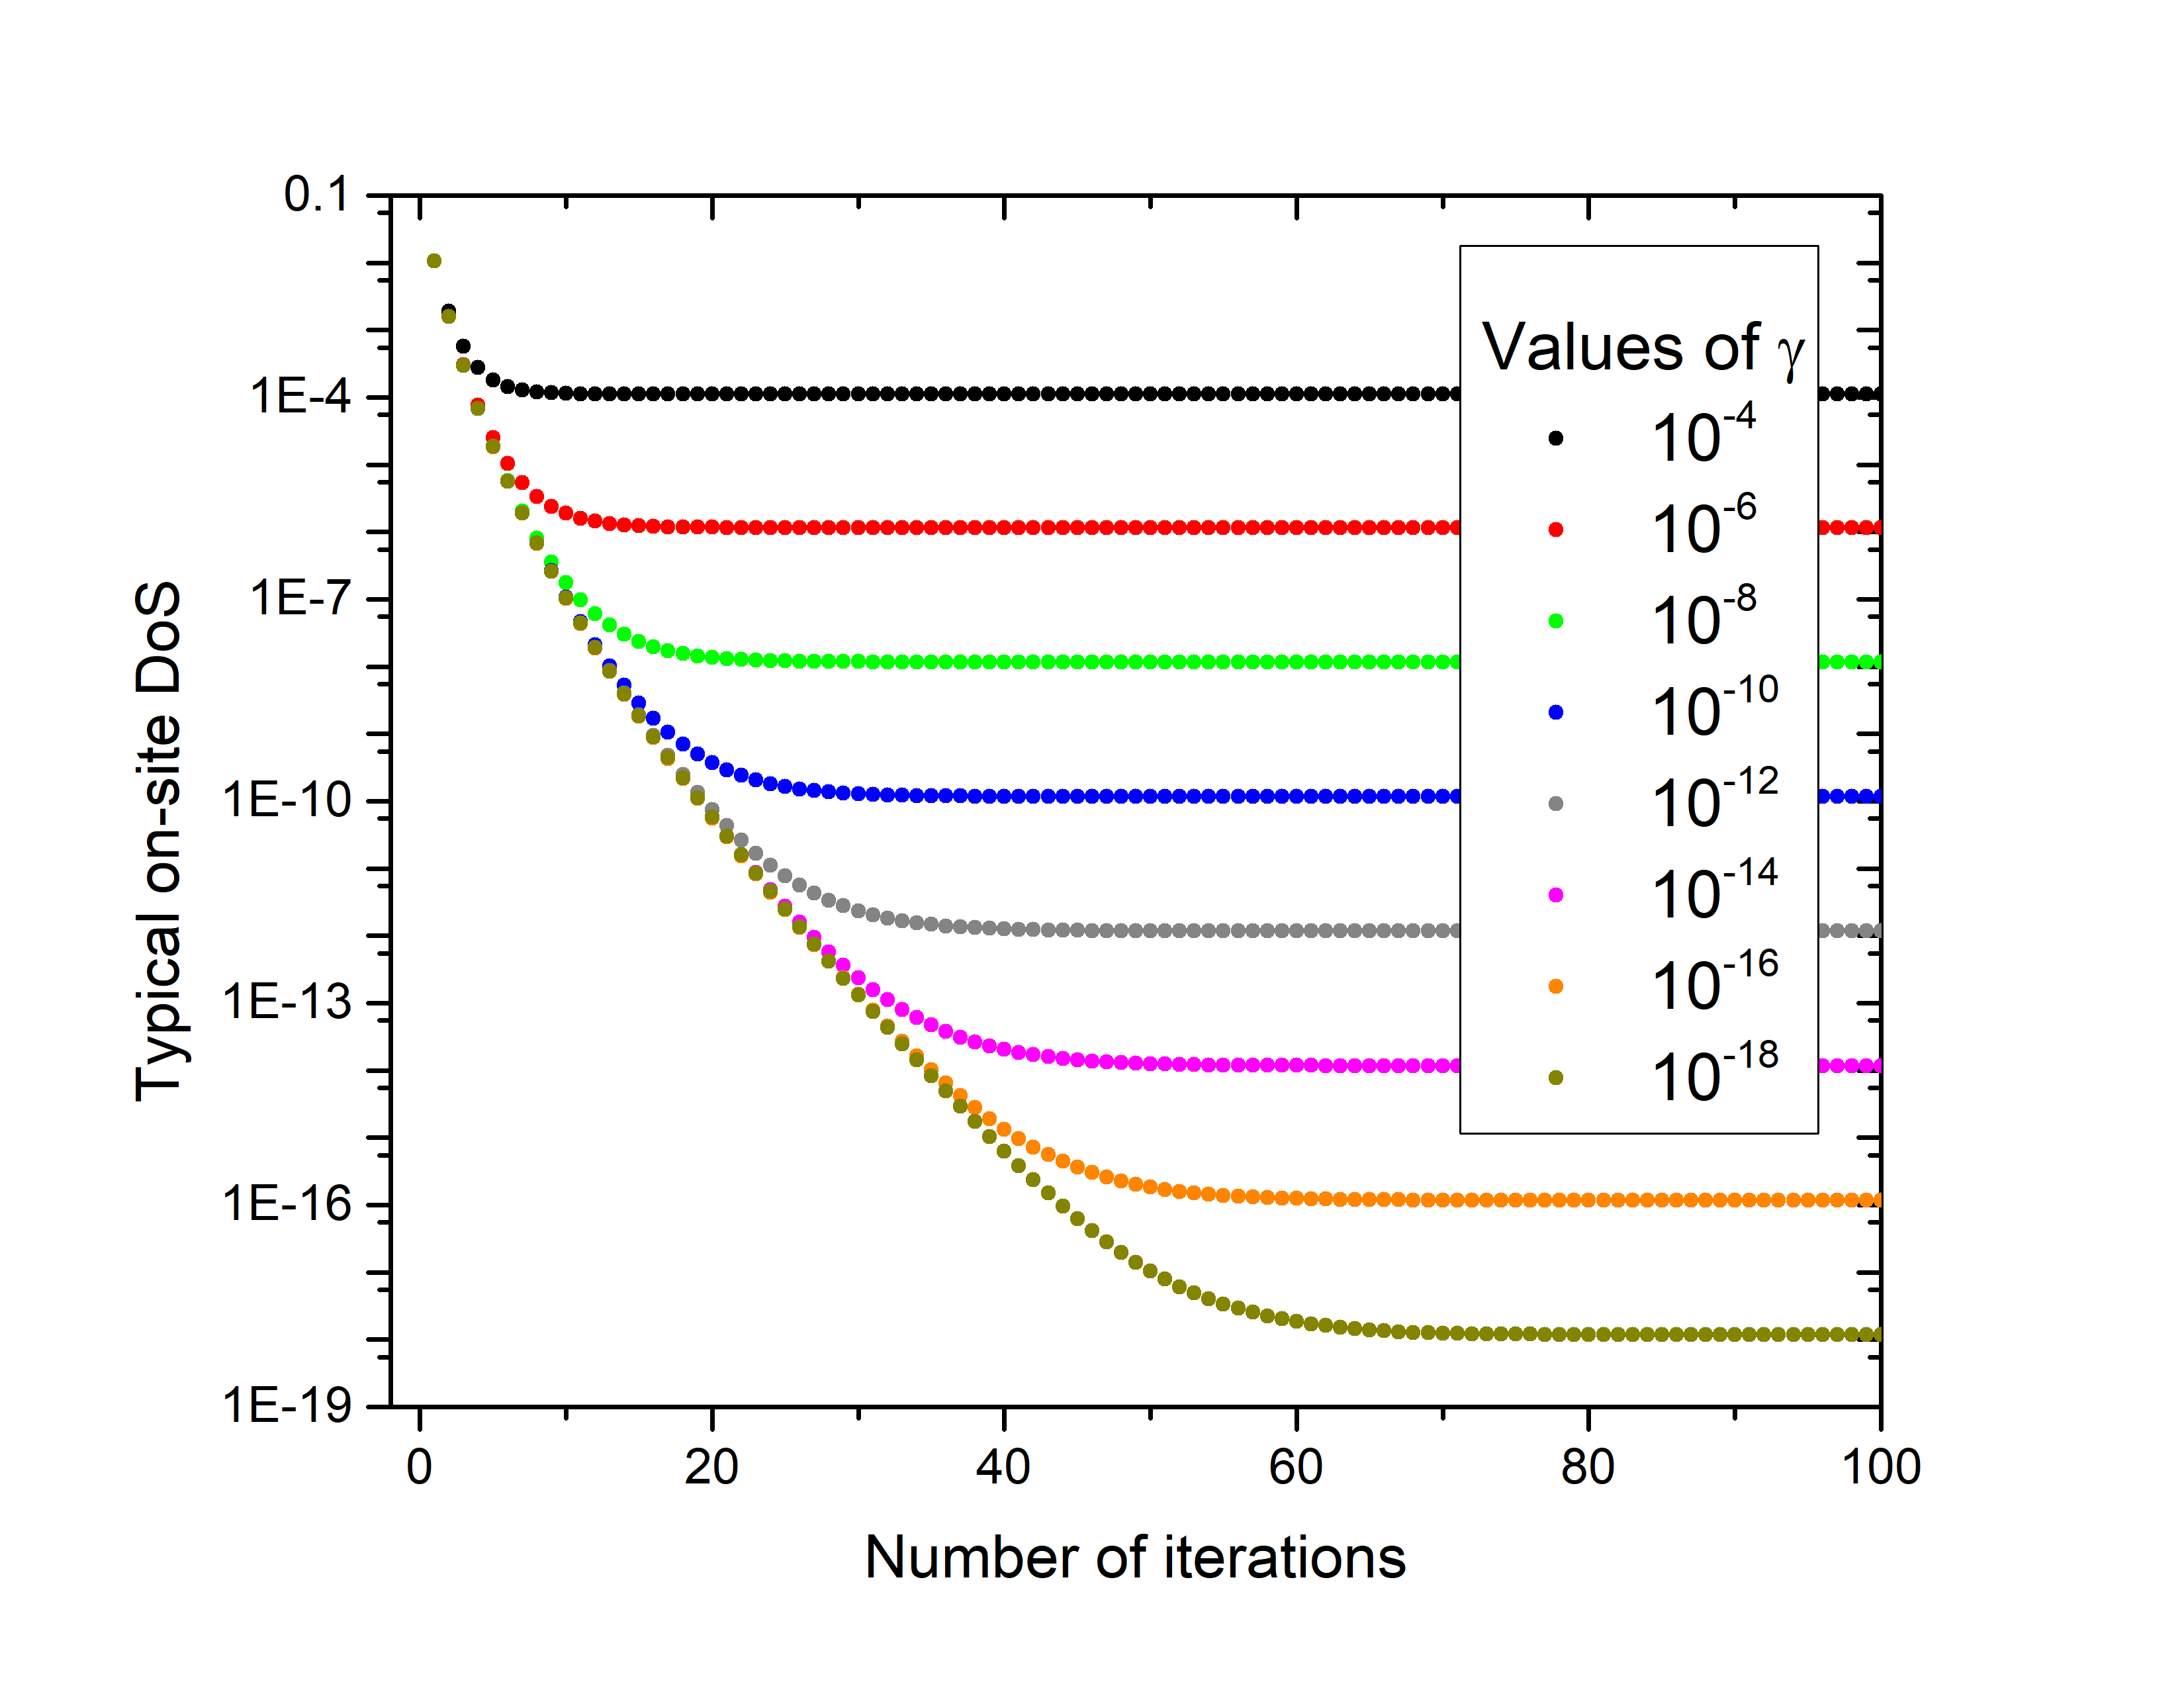
\includegraphics[width=0.85\textwidth]{Typical_convergence_various_gamma.png}
	\caption{Зависимость средней $\langle \rho \rangle$ (сверху) и типичной $\exp \langle \ln \rho \rangle$ (снизу) плотности состояний от числа итераций алгоритма при различных значениях $\gamma$. Размер выборки $M = 2^{26} \approx 6.7 \cdot 10^{8}$. Физические параметры симуляций см. в тексте.}
\end{figure}

\begin{figure}[h!p]
	\label{fig:Mean_convergence_for_various_M}
	\centering
	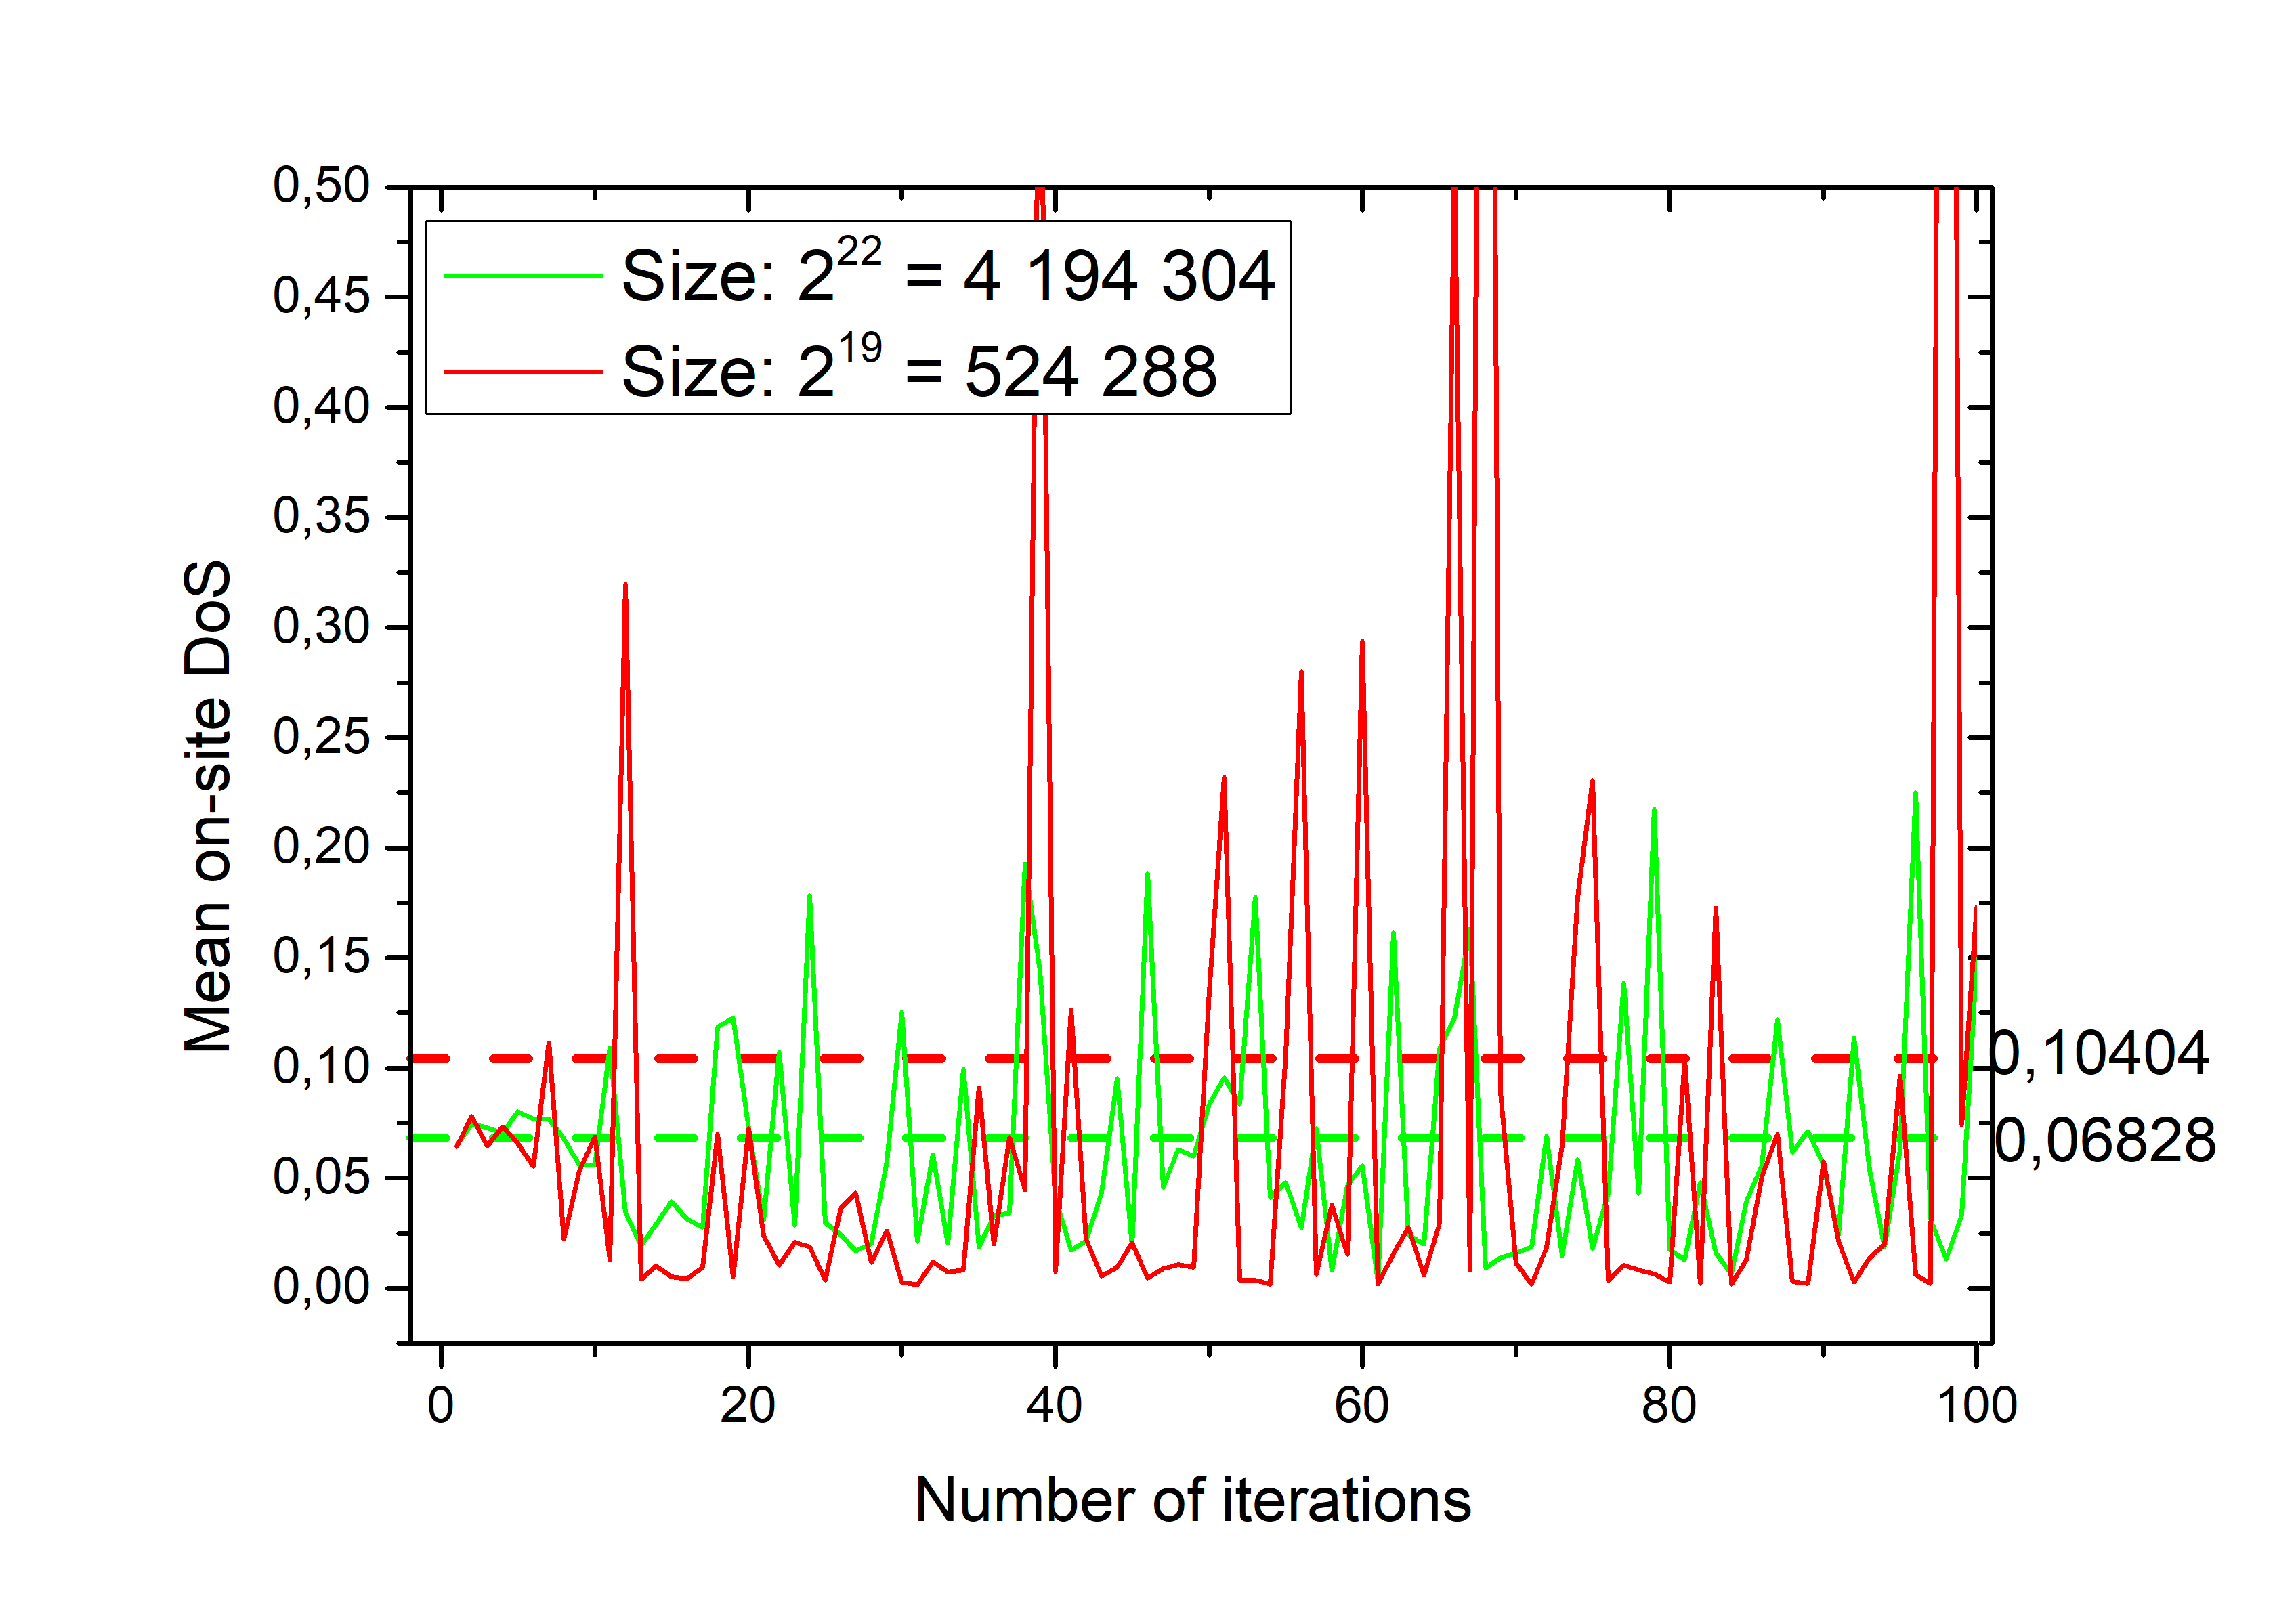
\includegraphics[width=0.8\textwidth]{Mean_convergence_for_various_M.png}
	\caption{Зависимость средней плотности состояний $\langle \rho \rangle$ от числа итераций алгоритма при двух различных значениях $M$ (указаны на рисунке). Значение регуляризации $\gamma = 10^{-7}$. Для сравнения на рисунке приведены также оценки для итерационного среднего вида $\overline{\langle \rho \rangle}$. Физические параметры симуляций см. в тексте.}
\end{figure}

Ключевые особенности приведённых зависимостей следующие:
\begin{itemize}
	\item имеется характерное время установления стационарного режима как для среднего, так и для типичного. Этот режим в неизменном виде наблюдается сколь угодно долго (в серии симуляций на Рис. \ref{fig:Convergence_for_various_gamma} максимальное число итераций составляет $N = 1000$).
	\item Факт совпадения времён установления среднего и типичного косвенно свидетельствует в пользу того, что данное время является характерным для установления всего распределения. Численные опыты с меньшим размером выборки (здесь не приведены) подтверждают это предположение.
	\item Время установления зависит от $\gamma$, причём зависимость на качественном уровне имеет степенной характер. Подробные исследования этой зависимости не проводились.
	\item В стационарном режиме среднее испытывает сильные флуктуации (в несколько порядков), амплитуда которых возрастает с уменьшением $\gamma$. На практике эти флуктуации означают, что среднее в этом алгоритме является плохо определённой величиной, поэтому для оценки первого момента распределения предлагается усреднять среднюю плотность состояний $\exp \overline{\ln \langle \rho \rangle}$ по итерациям.
	\item Значение среднего, около которого происходят флуктуации, и размах флуктуаций также сильно чувствительно к размеру выборки $M$. Более того, при малых размерах выборки стационарная динамика демонстрирует наличие резких пиков среднего, которые длятся ровно одну итерацию. Качественные комментарии, объясняющие это поведение, мы дадим чуть позже, когда разберёмся с влиянием параметров $\gamma, M$ на всё стационарное распределение.
	\item Напротив, типичное значение практически не испытывает флуктуаций и слабо чувствительно к размеру выборки, а потому является хорошо определённой характеристикой всего распределения. В купе с уже сказанным, это сильно облегчает задачу по выяснению степени сходимости алгоритма по числу итераций --- достаточно просто следить за установлением типичного (вместо того, чтобы хранить на каждой итерации всё распределение из $\sim 10^8$ значений). 
	\item Также важно заметить, что среднее и типичное являются сильно зависящими от $\gamma$. Это характерный признак отсутствия насыщения по $\gamma$. Поэтому в дальнейшем при предъявлении различного рода зависимостей будут приводиться версии этой зависимости при различных значениях $\gamma$, чтобы можно было судить о степени насыщения.
\end{itemize}

\subsubsection{Влияние параметров $M ,\gamma$  на форму стационарного распределения}
На Рис. \ref{fig:DOS_disribution_for_various_gamma} приведены формы стационарного распределения для двух различных значений $\gamma$, а на Рис. \ref{fig:DOS_disribution_for_various_M} --- для различных значений размера выборки $M$. Постоянные физические параметры всё те же: $K = 2, g = 0.15, \Delta = 2 \exp \left\{ -\frac{1}{g} \right\}$.
 
\begin{figure}[h!]
	\label{fig:DOS_disribution_for_various_gamma}
	\centering
	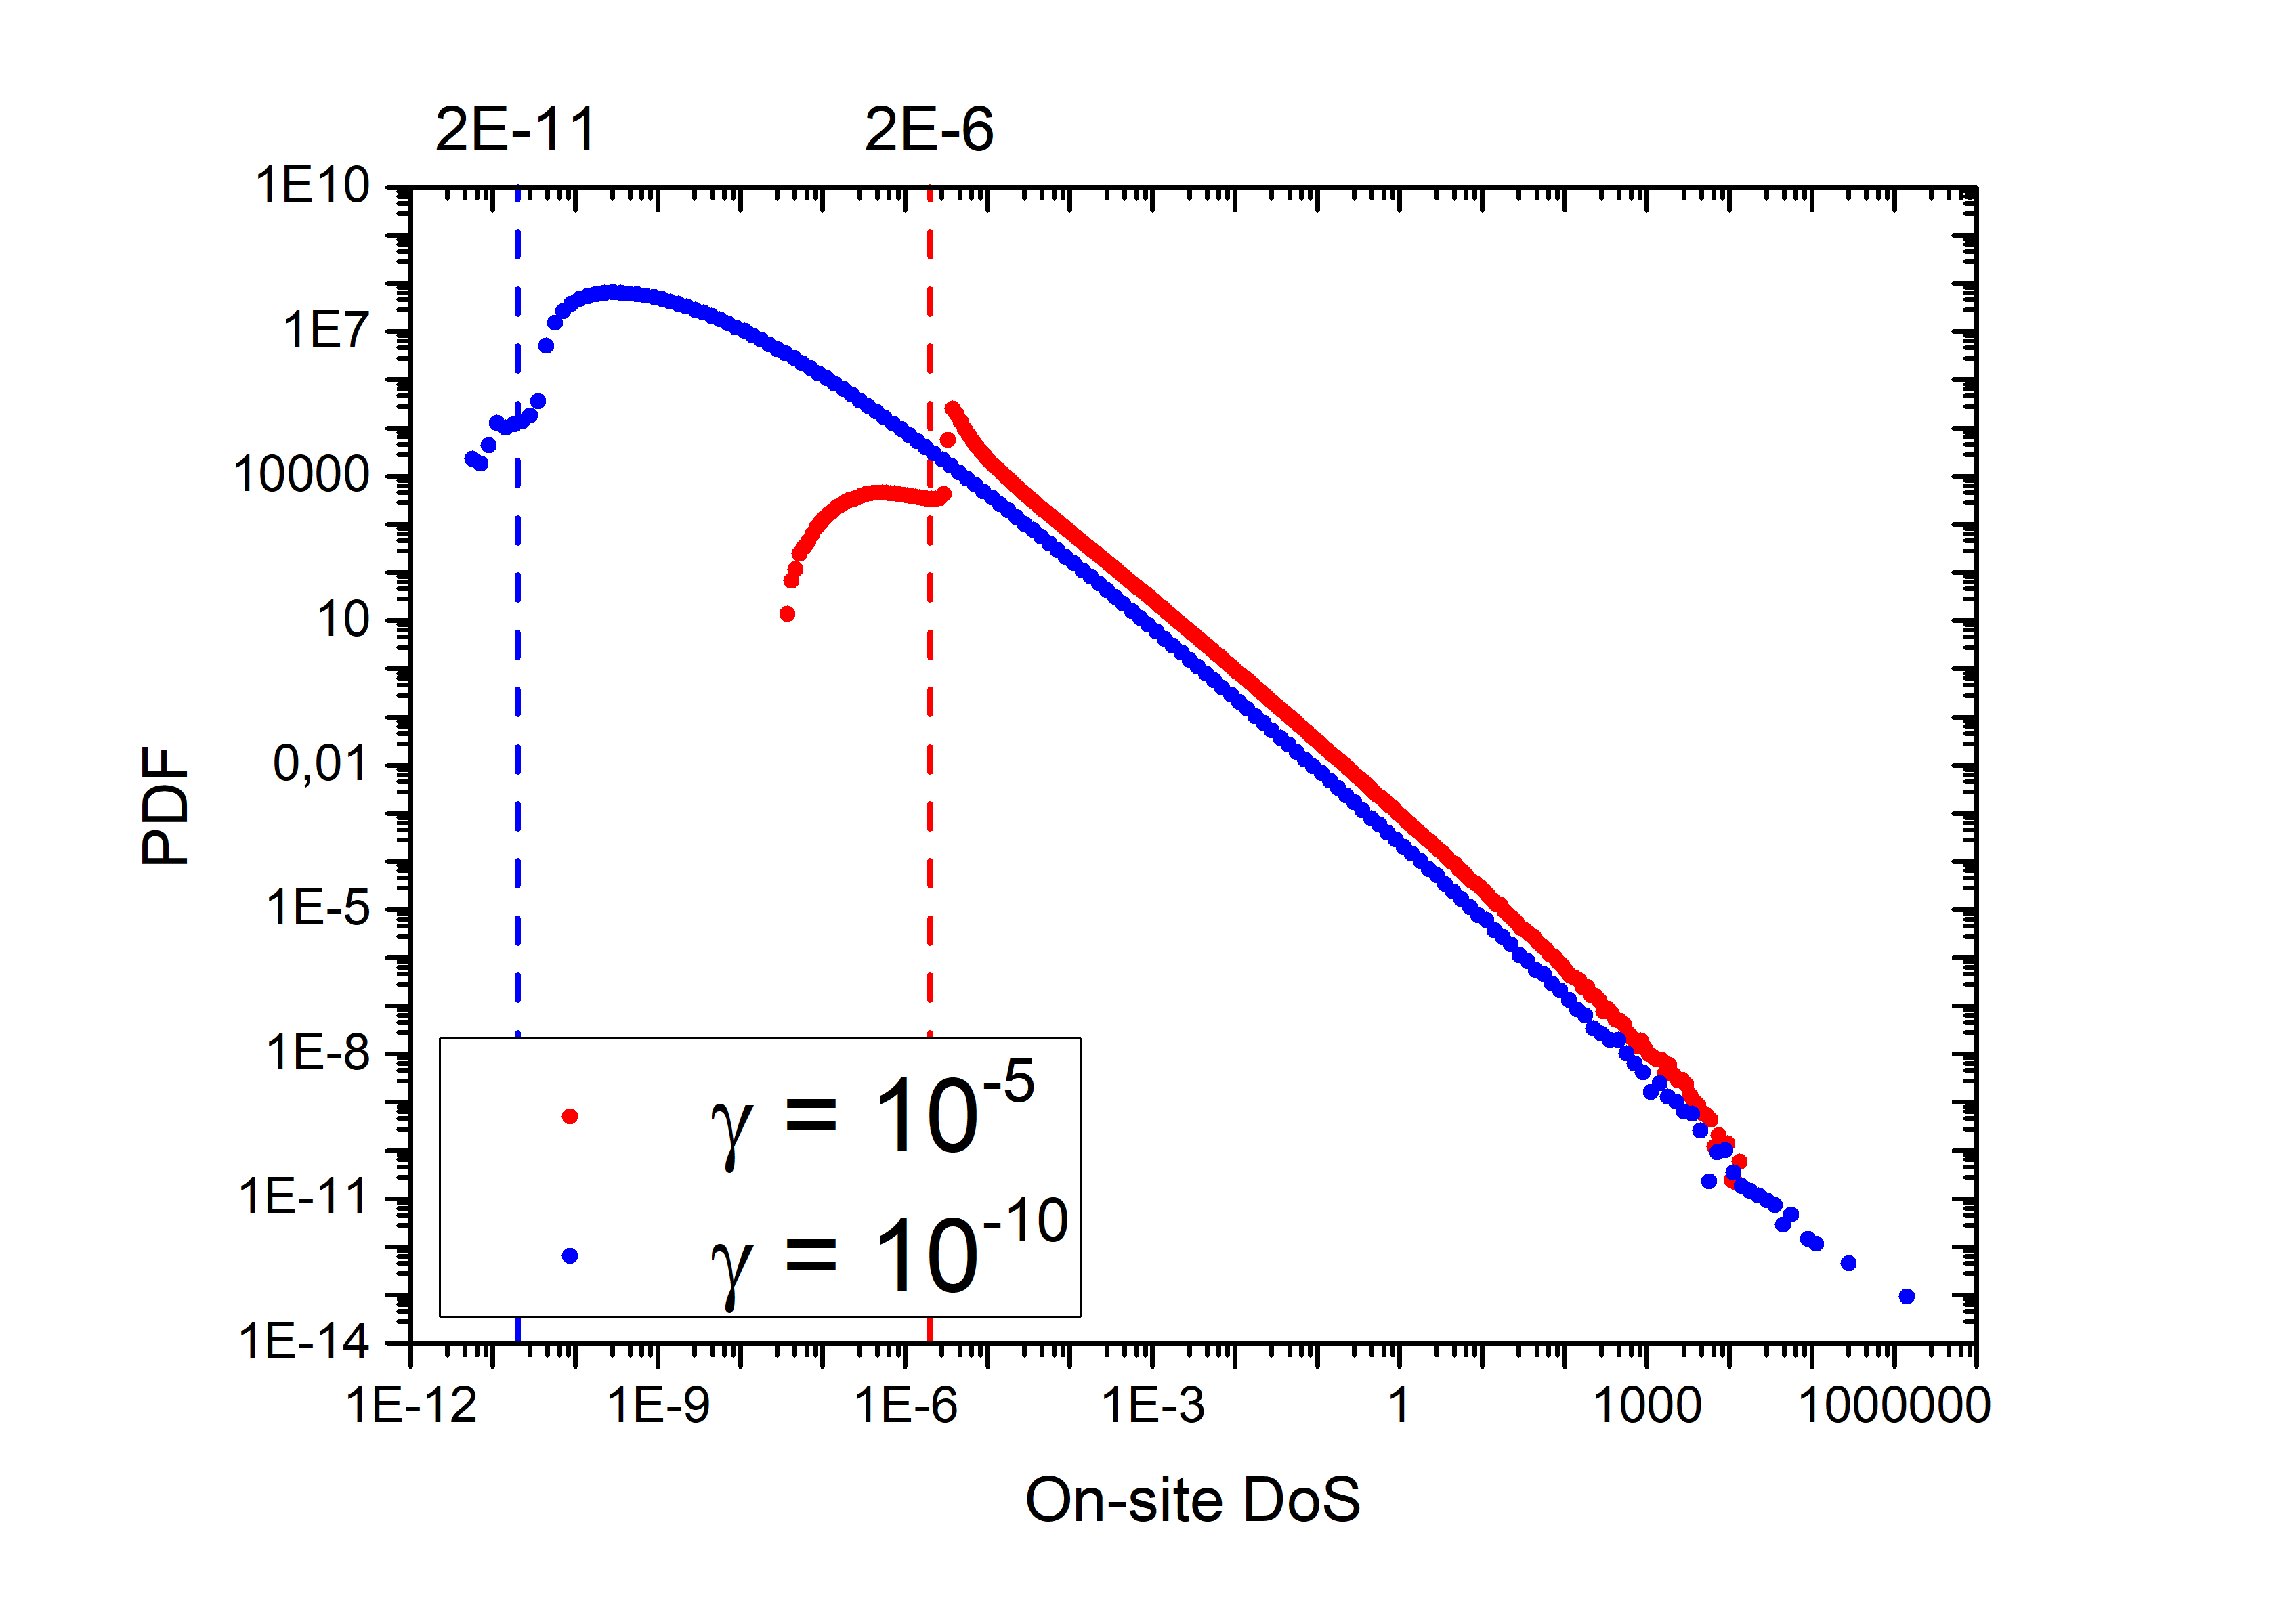
\includegraphics[width=0.8\textwidth]{DOS_disribution_for_various_gamma.png}
	\caption{Форма стационарного распределения при двух различных значениях параметра $\gamma$ (указаны на рисунке). Размер выборки $M = 2^{25} \approx 3.4 \cdot 10^8$. Значения физических параметров см. в тексте}
\end{figure}

\begin{figure}[h!]
	\label{fig:DOS_disribution_for_various_M}
	\centering
	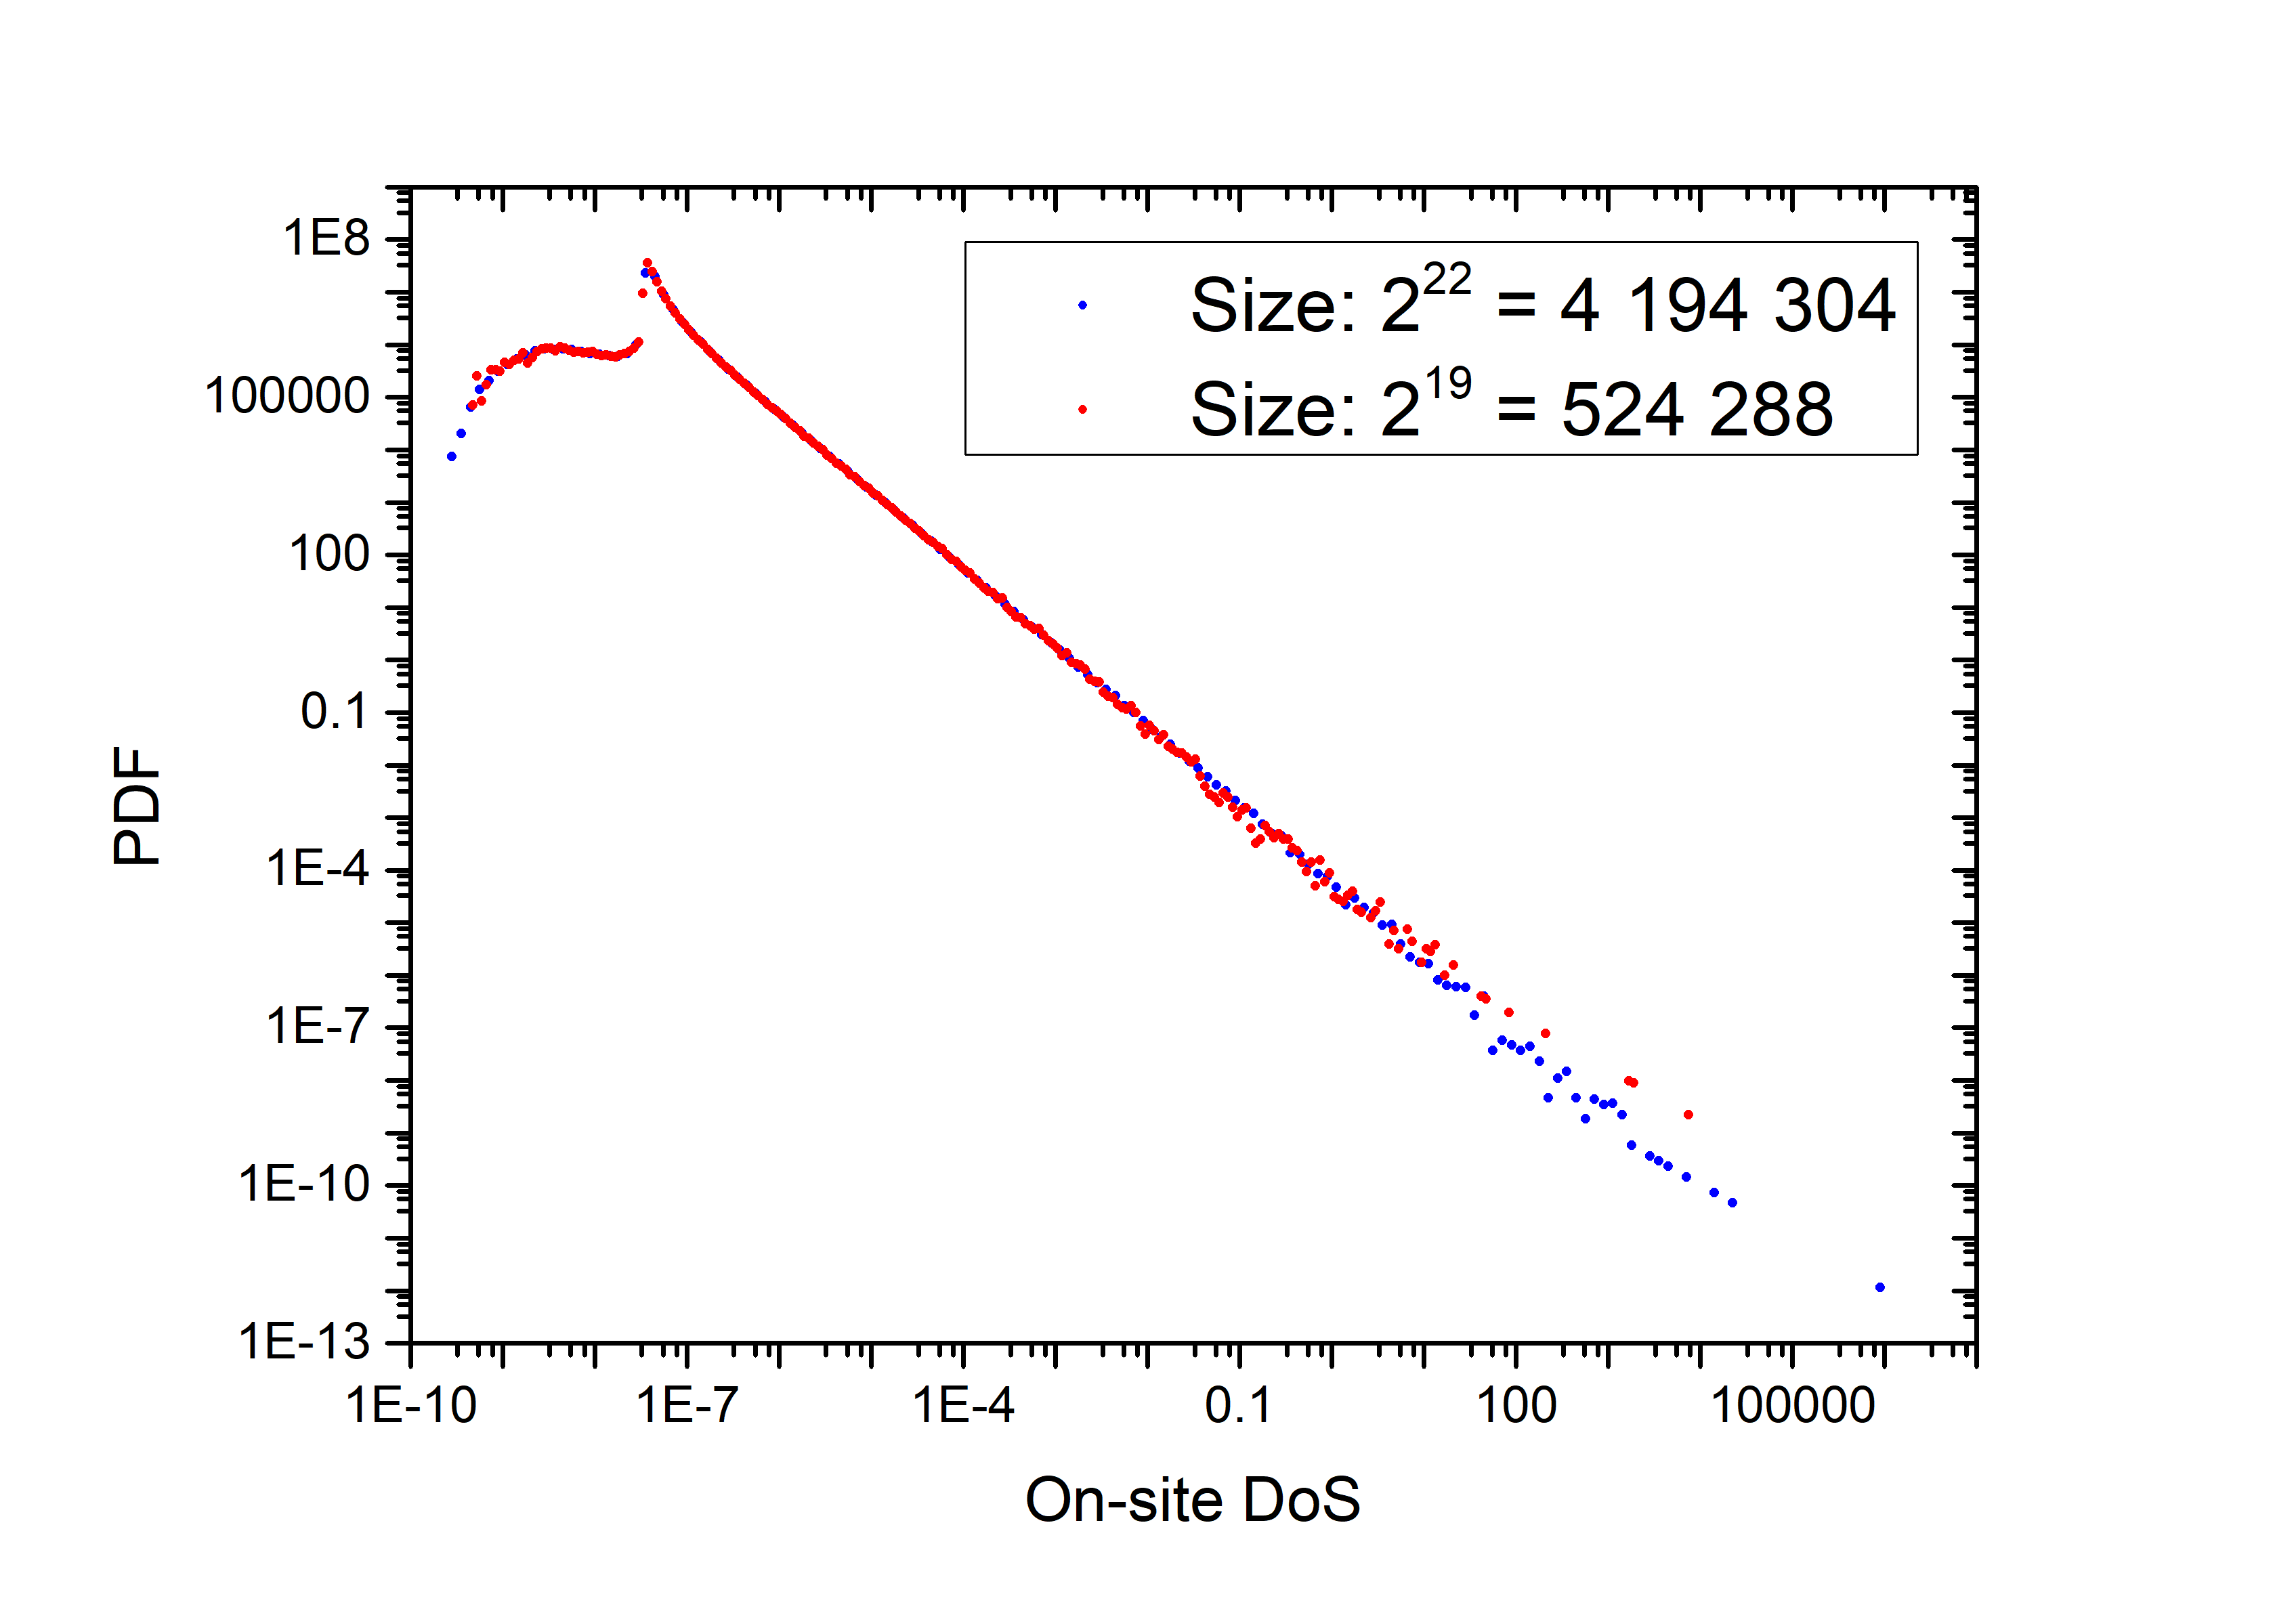
\includegraphics[width=0.8\textwidth]{DOS_disribution_for_various_M.png}
	\caption{Форма стационарного распределения при двух различных значениях параметра $M$ (указаны на рисунке). Значение параметра регуляризации $\gamma = 10^{-7}$. Значения физических параметров см. в тексте}
\end{figure}

Данные зависимости демонстрируют следующие качественные детали влияние параметров $M, \gamma$ на распределение:
\begin{itemize}
	\item При недостаточно малом $\gamma$ этот параметр создаёт резкую отсечку распределения на некотором значении, линейно зависящем от $\gamma$. Это легко понять, посмотрев непосредственно на формулы популяционной динамики \eqref{eq:Population_dynamics_final_equations} и сделав оценки для конкретных чисел:
	\begin{itemize}
		\item значений, больших по модулю, чем 
		$$\frac{g}{K \gamma \Delta} \sim 3 \cdot 10^{8}$$
		возникнуть не может в принципе (это соответствует строго нулевой действительной части и минимально возможному значению мнимой части знаменателя).
		\item В таком случае на следующей итерации значение модуля не может быть меньше
		$$ \left[ \frac{g}{K \gamma \Delta} K \right]^{-1} = \frac{\gamma \Delta}{g} \sim 2 \cdot 10^{-2} \gamma$$
		что мы и наблюдаем на практике с точностью до порядка.
	\end{itemize}
	Эти рассуждения также показывают, что среди экстремальных значений в выборке будет наблюдаться небольшое чередование по номеру итераций между большими и малыми значениями.
	\item Малый размер выборки, как и следует ожидать, оказывает обедняющее воздействие качество статистики на очень больших и очень малых значения плотности состояний. Как мы видели выше, статистика больших и малых значений в рамках этого алгоритма являются связанными: если размер выборки недостаточен для воспроизведения статистически значимых образцов одной области --- тоже самое произойдёт с другой. 
	\item Заметим, что поведение формы распределения объясняет характер поведения среднего и типичного по отношению к различным $\gamma, M$:
	\begin{itemize}
		\item как подсказывает степенная в широких пределах форма распределения (на ней мы ещё остановимся далее), в величину среднего дают доминирующий вклад экстремальные значения в выборке, а потому плохое воспроизведение очень больших значений плотности -- будь то по недостаточно малого $\gamma$ или небольшого $M$ -- приводит к неправильному значению среднего. Также описанные выше рассуждения о чередовании экстремальных значений очевидным образом объясняют наличие в стационарной динамике пиков длинной в одну итерацию.
		\item типичное значение, в отличие от среднего, нечувствительно к <<выбросам>> экстремальных значений, что объясняет слабую чувствительность типичного к размерам выборки.
		Однако, поскольку недостаточно малая $\gamma$ одинаково сильно обрезает оба масштаба, то простой оценкой вида:
		$$
		\rho_{typ} \sim \exp\left\{ \int \limits_{ x_{small} = \sharp \gamma }^{ x_{large} = \sharp \gamma^{-1} } \frac{dx}{x^n} \ln x \right\} \sim \gamma  \exp \left\{ \sharp x_{small}^{1-n} + \sharp x_{large}^{1-n} \right\}
		$$
		легко объяснять, почему типичное также чувствительно к регуляризации $\gamma$.
	\end{itemize}
\end{itemize}